\documentclass{report}

\usepackage{graphicx}
\usepackage[english]{babel}
\usepackage[utf8x]{inputenc}
\usepackage[T1]{fontenc}
\usepackage{sectsty}
\usepackage{pdfpages}
\usepackage[section]{placeins}
\usepackage{float}% If comment this, figure moves to Page 2
\usepackage{listings}
\usepackage{caption}
\usepackage{subcaption}

\begin{document}

\chapter{Testability}
\section{Overview}
Testability is concerned with ensuring the software architecture eases the work of testers. The way in which the software is designed should make it easy for precise tests to be developed to measure how successful the software was made.
\begin{itemize}
\item NOT the same as testing itself
\item Software architecture is structured in a way so that desired testing can take place
\item Testability is often determined by the code structure itself rather than the connector/component or deployment view
\item Consider the code modules and the dependencies between them that are used to build up the components
\end{itemize}

\section{General Scenario of Testing}
\begin{itemize}
\item   
   \textbf{Source:}
   Can think of it as who is doing the testing:
   \begin{itemize}
   \item unit testers
   \item integration testers
   \item system testers
   \item acceptance testers
   \item end users
   \end{itemize}
   These tests can be run manually or using automated testing tools
   
\item 
   \textbf{Stimulus:} 
   Why is the set of tests being executed? 
   Could be due to:
   \begin{itemize}
   \item completion of a certain part of the code, or of an entire system
   \item complete integration of subsystem into larger system
   \item completion of entire system
   \item time to deliver the system to the customers
   \end{itemize}
   
    
\item 
   \textbf{Environment:}
   Which environment we are dealing with:
   \begin{itemize}
   \item Design time
   \item Development time
   \item Compile time
   \item Integration time
   \item Deployment time
   \item Run time
   \end{itemize}  

\item
   \textbf{Artifacts:}
   The portion of the system that is being tested

\item 
   \textbf{Response:}
   What is the outcome of running the tests:
   \begin{itemize}
   \item Execute test suite and capture results
   \item Capture activity that resulted in the fault
   \item Control and monitor the state of the system
   \end{itemize} 

\item 
   \textbf{Response Measure:}
   How exactly we will measure the results and if we were successful in the testing
   Could be:
   \begin{itemize}
   \item Find a fault or type of faults
   \item Achieve a certain percentage of code coverage
   \item Time limit for running the tests
   \end{itemize} 
\end{itemize}

Figure 1.1 on the next page shows an example of this general scenario.
\begin{figure}[h]
\begin{center} 
    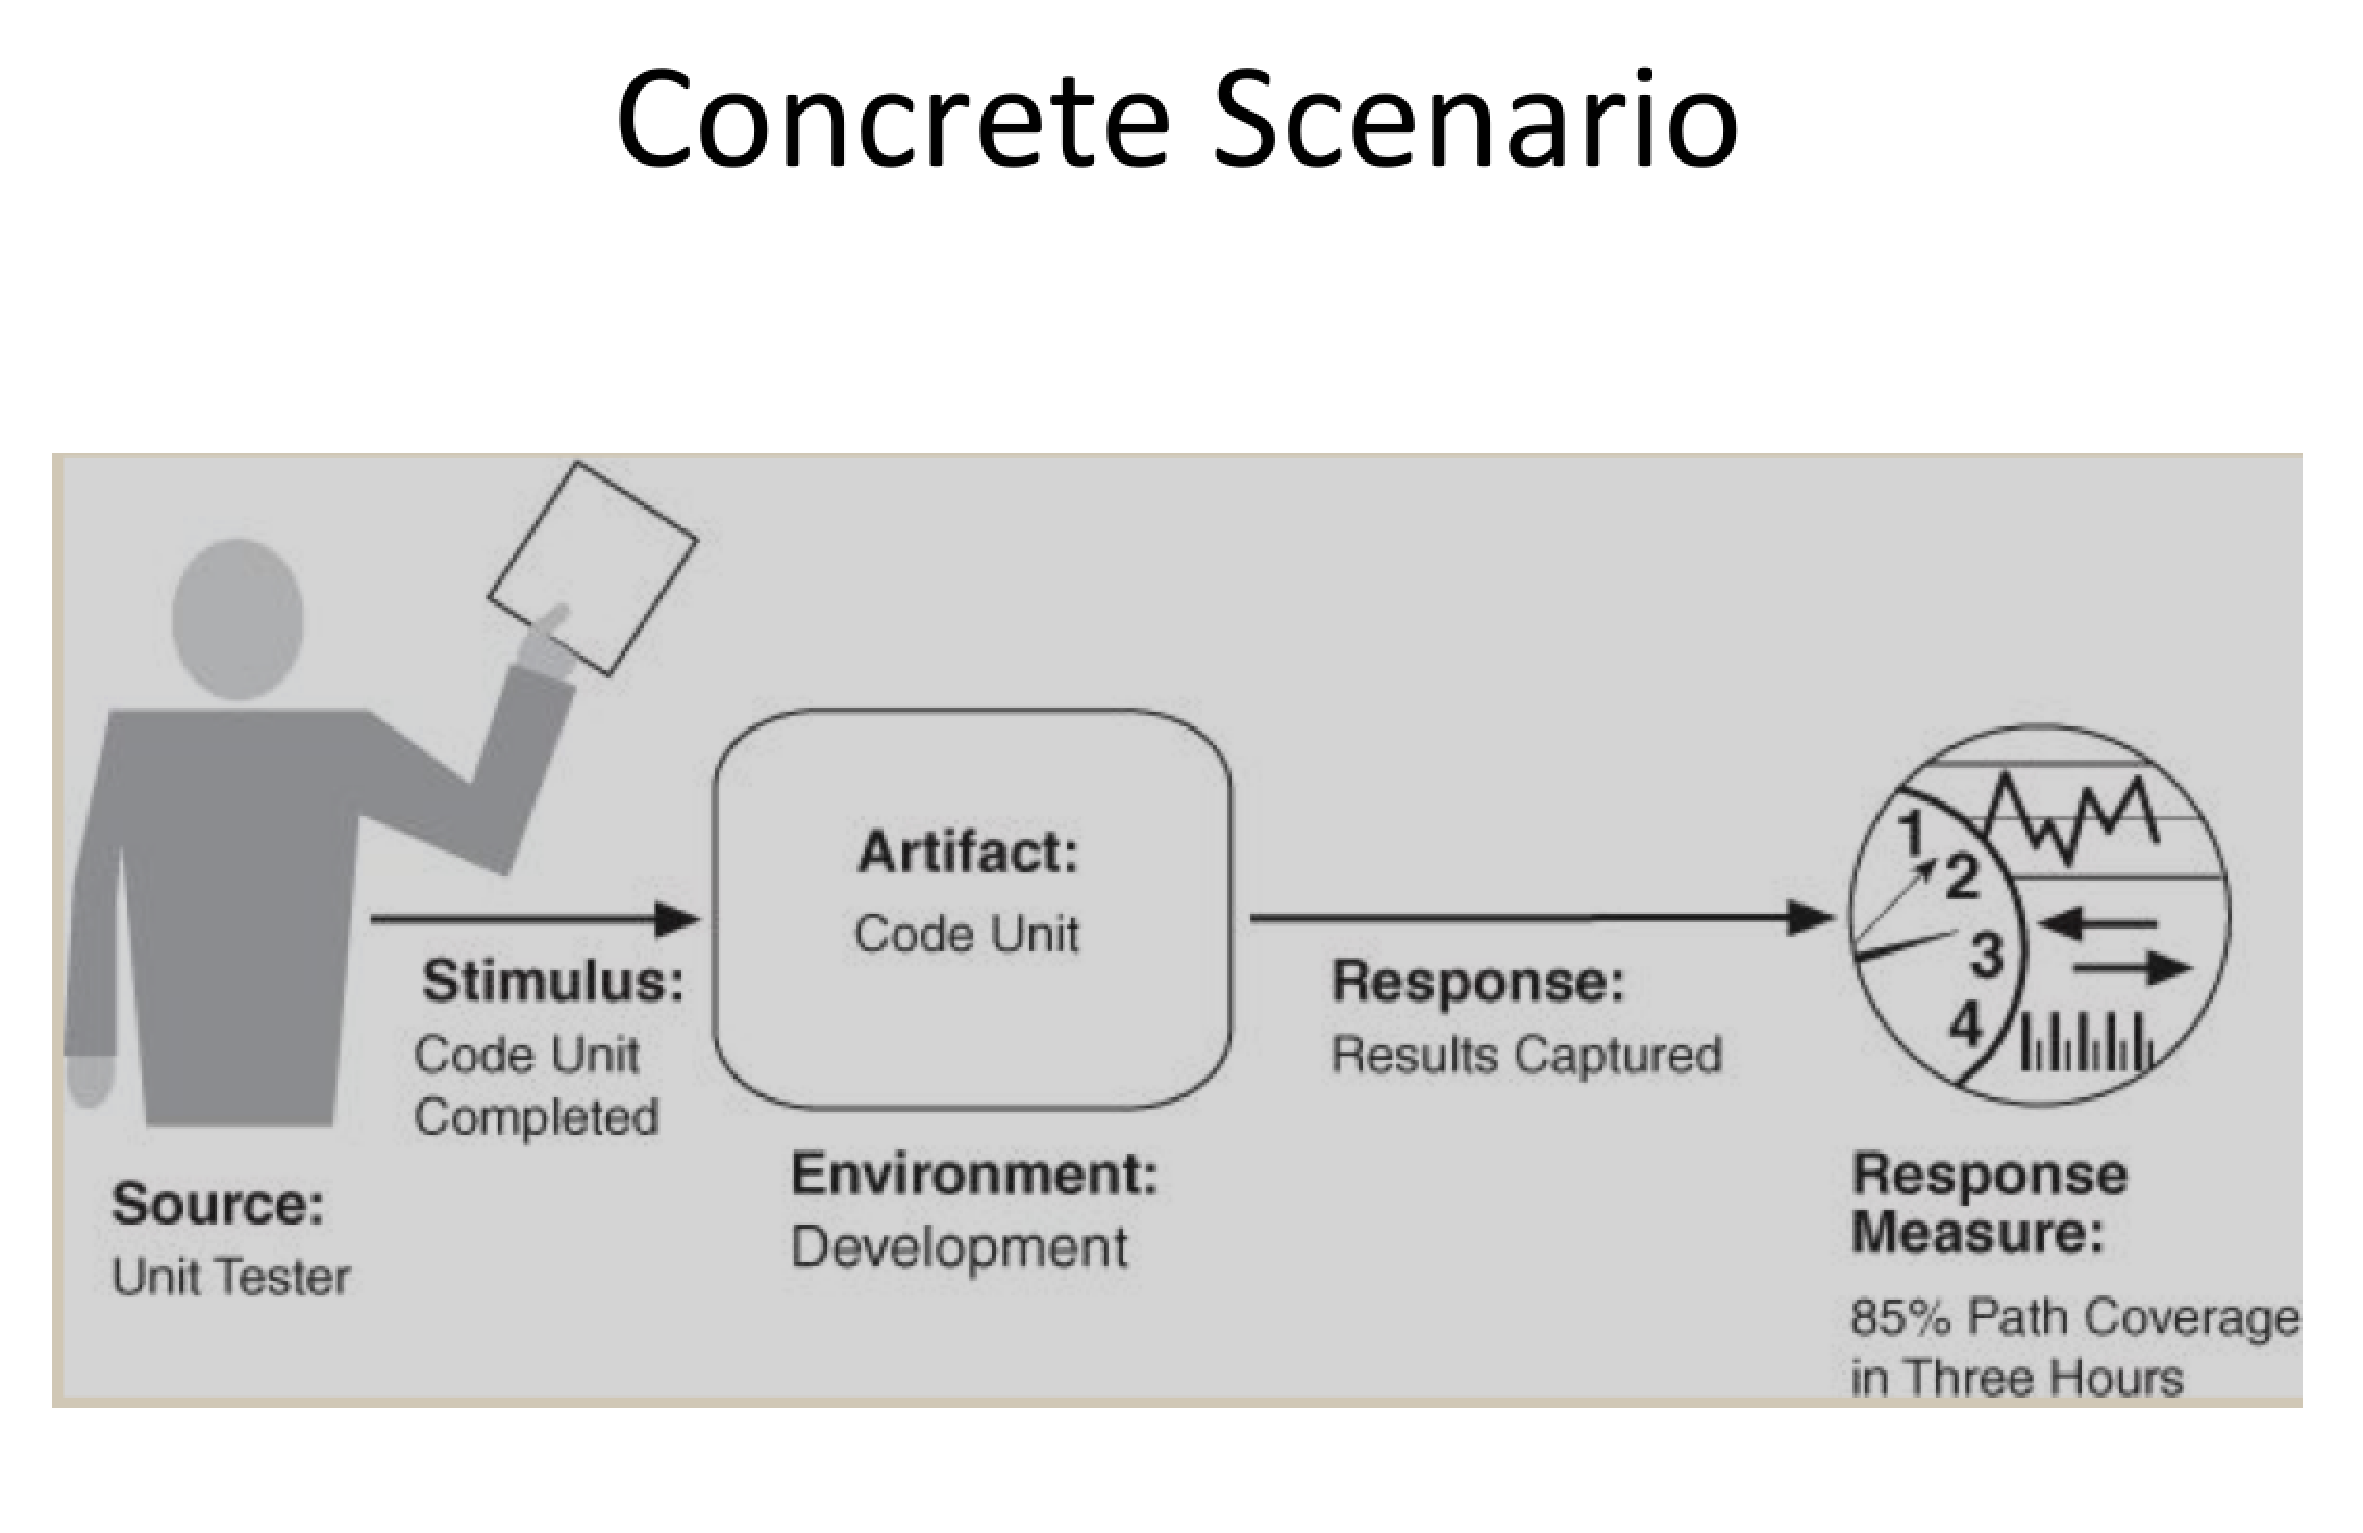
\includegraphics[scale=0.8,width = 15cm, height = 12cm]{images/n05at-zq1xe.pdf}
    \caption{An example of such a scenario}
\end{center}
\end{figure}

Testability deals with making this process easier to carry out.

\section{Main Tactics Towards Increasing Testability}
\begin{itemize}
\item Limit complexity in modules themselves - for example, split a large, complex module into smaller, less complex ones
\item Limit complexity in system structure - for example, introduce specific interfaces in a system that give us better access to a log database 
\item Limit nondeterminism
\end{itemize}


\section{Checklist Towards Achieving Testability}
During testing, tester has to control and observe the state of the system.

\begin{itemize}
\item
\textbf{Allocation of responsibilities:}
This means determining which system responsibilities are most critical and thus need the most testing.
Make sure that system responsibilities have been created to actually perform the testing and capture the results, capture(log) activity that resulted in fault or unexpected behaviour, control and observe relevant system state for testing.

\item
\textbf{Coordination Model:}
Ensure system's coordination and communication mechanisms
support the execution of the test suite,
support capturing activity that resulted in a fault,
support injection and monitoring of state, and
do no introduce unecessary nondeterminism

\item
\textbf{Data Model:}
Determine the major data abstractions that must be tested to ensure the correct operation of the system.

\item
\textbf{Mapping Among Architectural Elements:}
Determine how to test possible mappings of architectural elements so that the desired test response is achieved.

\item
\textbf{Resource Management:}
Ensure that there are sufficient resources available to execute the test suite and capture the results. 
Ensure test environment is representative of the environment in which the system will run in.

\item
\textbf{Binding Time:}
Ensure that components that are bound later than compile time can be tested in the late-bound context.

\item
\textbf{Choice of Technology:}
Determine what technologies are available to help achieve the testability scenarios that apply to your architecture. 
\end{itemize}

\section{Summary}
Testability becomes increasingly important in an environment where development is test driven. The main ways we can improve testability is via changing the observability of phenomena or by limiting complexity.

\chapter{Modifiability}
\section{Overview}
Modifiability is concerned with how easy it is to make changes to the system if this is required. So, for example, having a lot of hard coded values would not make a system very modifiable.

It's not about the actual modifying but with how easy it would be to do the modifying.
It is very important for a system to be modifiable because changes can be very costly to make.

\section{Four key questions that are asked when making a system:}
1)   What can change?\newline
2)   How likely is something to change?\newline
3)   When, where, how, and by whom will the change be made?\newline
4)   What is the cost of making these changes? \newline

\section{A specific scenario with same "general scenario" terms used as in the testability section:}

Source: Developer \newline
Stimulus: Wishes to change the UI \newline
Artifact: The code itself \newline
Environment: Design time \newline
Response: Change made and unit tested \newline
Response Measure: This should all be done in 3 hours \newline

\section{Important Terms}
\begin{itemize}
\item \textbf{Cohesion -} refers to the degree to which the elements inside a module belong together.
\item \textbf{Semantic coherence –} all the responsibilities in a layer work together without too much reliance on other layers
\item \textbf{Coupling –} degree of interdependence between software modules
\item \textbf{Intermediary -} a program or set of programs that in some way evaluates, filters, modifies, or otherwise interjects some function between two end users or end-use programs
\item \textbf{Binding -} generally refers to a mapping of one thing to another. In the context of software libraries, bindings are wrapper libraries that bridge two programming languages, so that a library written for one language can be used in another language.
\item \textbf{Deferred Binding -} When a modification is made by the developer, there is usually a testing and distribution process that determines the time lag between the making of the change and the availability of that change to the end user. Binding at runtime means that the system has been prepared for that binding and all of the testing and distribution steps have been completed. Deferring binding time also supports allowing the end user or system administrator to make settings or provide input that affects behavior.
\end{itemize}

\section{Tactics of Modifiability:}
\begin{itemize}
  \item \textbf{Reduce size of a module} – split it up
  \item \textbf{Increase cohesion within a module} – increase semantic coherence
  \item \textbf{Decrease the coupling in the module} – this can be done in the following ways:
   \begin{itemize}
   \item Encapsulate
   \item Use an intermediary
   \item Restrict dependencies
   \item Refactor
   \item Abstract common servies – think of OOP
   \end{itemize}
   \item \textbf{Defer binding} – we can use the “reduce coupling” tactics later in the process so that they   are more likely to be done by a computer rather than a human
\end{itemize}

\section{Checklist Towards Achieving Modifiability}
\begin{itemize}
\item
\textbf{Allocation of Responsibilities:}
Try to work out how things are likely to change – work out what responsibilities change.
Try to modularize so that change does not affect responsibilities that span many modules.

\item
\textbf{Coordination Model:}
See how changes are likely to affect coordination and make it so that most probable changes impact coordination across a small numebr of modules.  

\item
\textbf{Data Model:}
Data model changes impact as few modules as possible.

\item
\textbf{Mapping Among Architectural Elements:}
Look at potential changes and see if some may best be responded to by changing the mapping to elements.

\item
\textbf{Resource Management:}
Determine how a change in responsibility will change resource.

\item
\textbf{Binding Time:}
Control choice of binding times so there are not too many combinations to consider. Defer binding to later.

\item
\textbf{Choice of Technology:} 
Choose technologies that make the most likely changes easier – of course, balance with costs.
\end{itemize}

\section{Summary}
Summary:
For better modifiability:
1) Improve cohesion, reduce coupling
2) Use mechanisms that allow you to introduce change late in development cycle
3) Of course, take the cost of all these mechanisms into account

\chapter{Architectural Modeling:}
\section{Overview}
When building a software architecture, we want to ideally have control over the quality attributes (example – testability, modifiability, etc) and even to be able to predict how well our system will be able to do in each one in advance. 

So – we want to be able to build a predictive model of the software architecture and then use this model to predict the quality attributes – how well our software will perform on each of them.

\section{How the model looks like:}
1)  The beginning specifies the distribution of arrivals of service requests. \newline
2)  The queuing discipline \newline
3)  The scheduling algorithm  \newline
4)  Routing of messages coming from the algorithm  \newline
5)  The results – could be the quality attributes the model is predicting \newline

\section{MVC Model – model to test the “performance” quality attribute}
1) The view component will service the service requests at some rate.  \newline
2) The view translates these into service requests for the controller.  \newline
3) The there are service requests from the controller to the view, from the controller to the model, and from the model to the view component – all are interleaved.  \newline

If we have good estimates for all the different components of the model (distribution of external service demands, queuing disciplines, network latencies, transfer characteristics), then it can be a very good predictor of quality attributes.

\section{Main Quality Attributes and their Analysis Techniques}
The main quality attributes and their analysis techniques are:
\begin{itemize}

\item \textbf{Availability} – Markov models, statistical models \newline
Availability is a measure of software quality defined as MTBF / (MTBF + MTTR)
MTBF is Mean Time Between Failures
MTTR is Mean Time To Repair 

\item \textbf{Interoperability} – Conceptual framework 

\item \textbf{Modifiability} – Coupling and cohesion metrics, cost models

\item \textbf{Performance} – Queuing theory, real-time scheduling theory

\item \textbf{Security} – No architectural models

\item \textbf{Testability} – Component interaction metrics

\item \textbf{Usability} – No architectural models
\end{itemize}

Some QAs have good, well established analysis techniques, others do not,

\section{Types of Analysis}
\begin{itemize}
\item
\textbf{Thought experiment:} just a sort of discussion using informed people. 

\item
\textbf{Back of the envelope:} using very approximate techniques with unreliable assumptions

\item
\textbf{Checklist:} collated experience.

\item
\textbf{Analytic Model:} based on sound abstractions –heavily dependent on estimates being correct

\item
\textbf{Simulation:} higher level of detail – less analytic, more concrete 

\item
\textbf{Prototype:} approximate system in an experimental setup

\item
\textbf{Experiment:} fielded system, simulated load 

\item
\textbf{Instrumentation:} measuring the variable of interest
\end{itemize}

\section{Summary}
Architecture is the correct level to deal with quality attributes.
Analysis can be costly, depending on how accurate you want it to be.
Analysis throughout the lifecycle helps with decision taking.

\chapter{Lifecycle}
\section{Overview}
They impose some discipline on the development process – order stages and activities of the development process. Usually it's an ongoing process improvement cycle that focuses on making this process better.

\section{Typical Examples}
There are some typical stages of the software lifecycle.
\begin{figure}[h]
\begin{center} 
    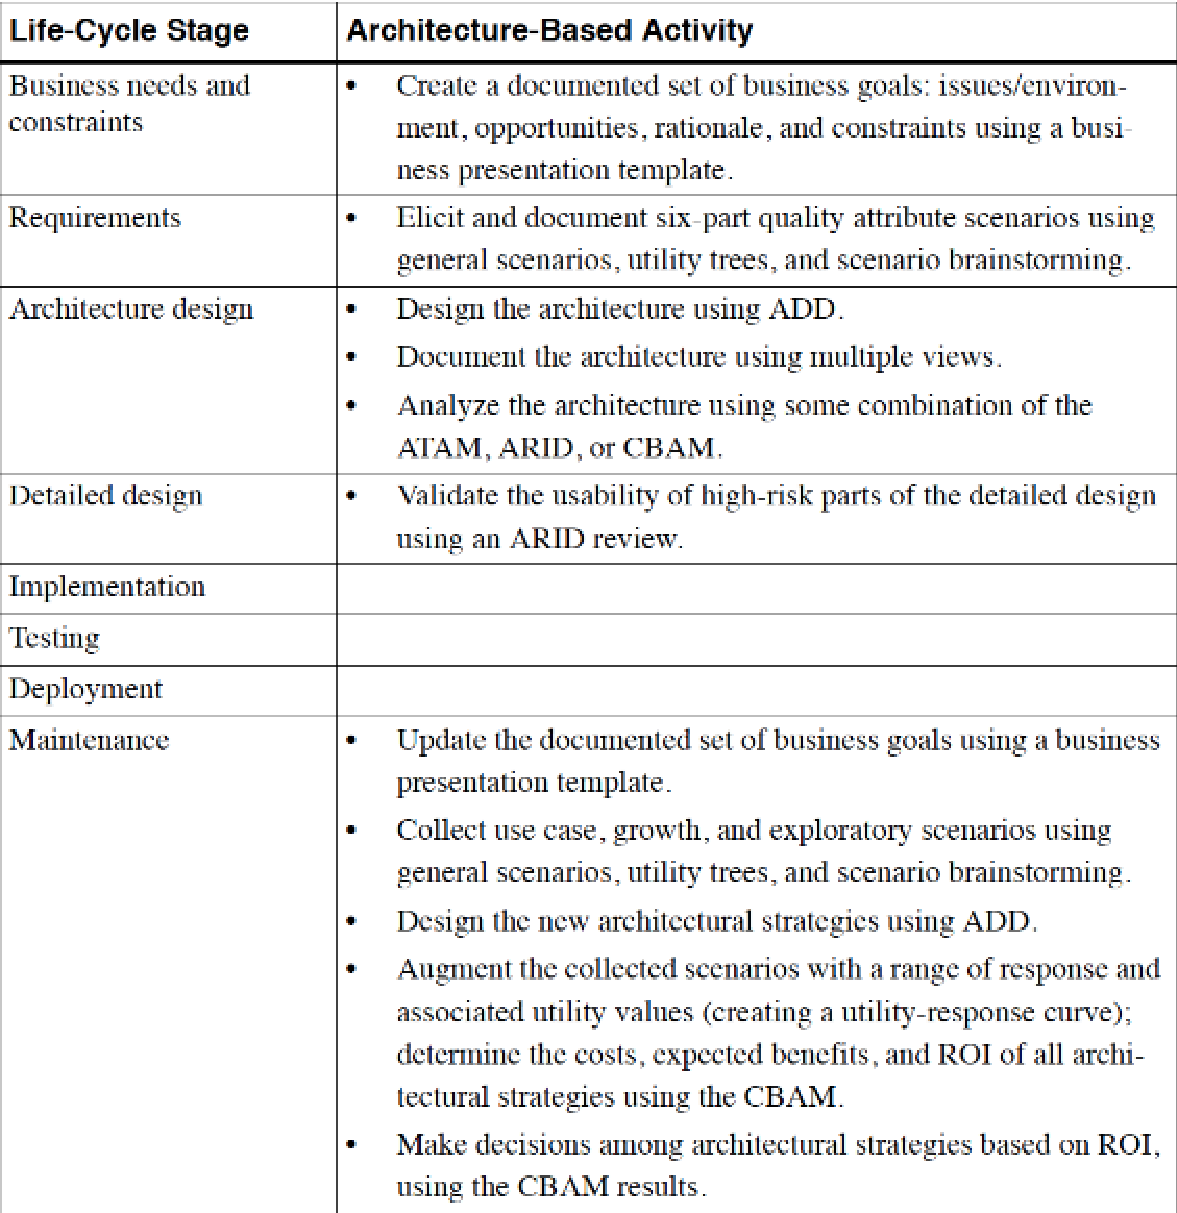
\includegraphics[scale=0.6,width = 15cm, height = 12cm]{images/LifecycleStages.pdf}
    \caption{A diagram showing the typical lifecycle stages and what software engineers do to the architecture at each stage.}
\end{center}
\end{figure}

The images on the next few pages show the typical stages of the software lifecycle and then typical examples of different software lifecycles.

\begin{figure}[h]
\begin{center} 
    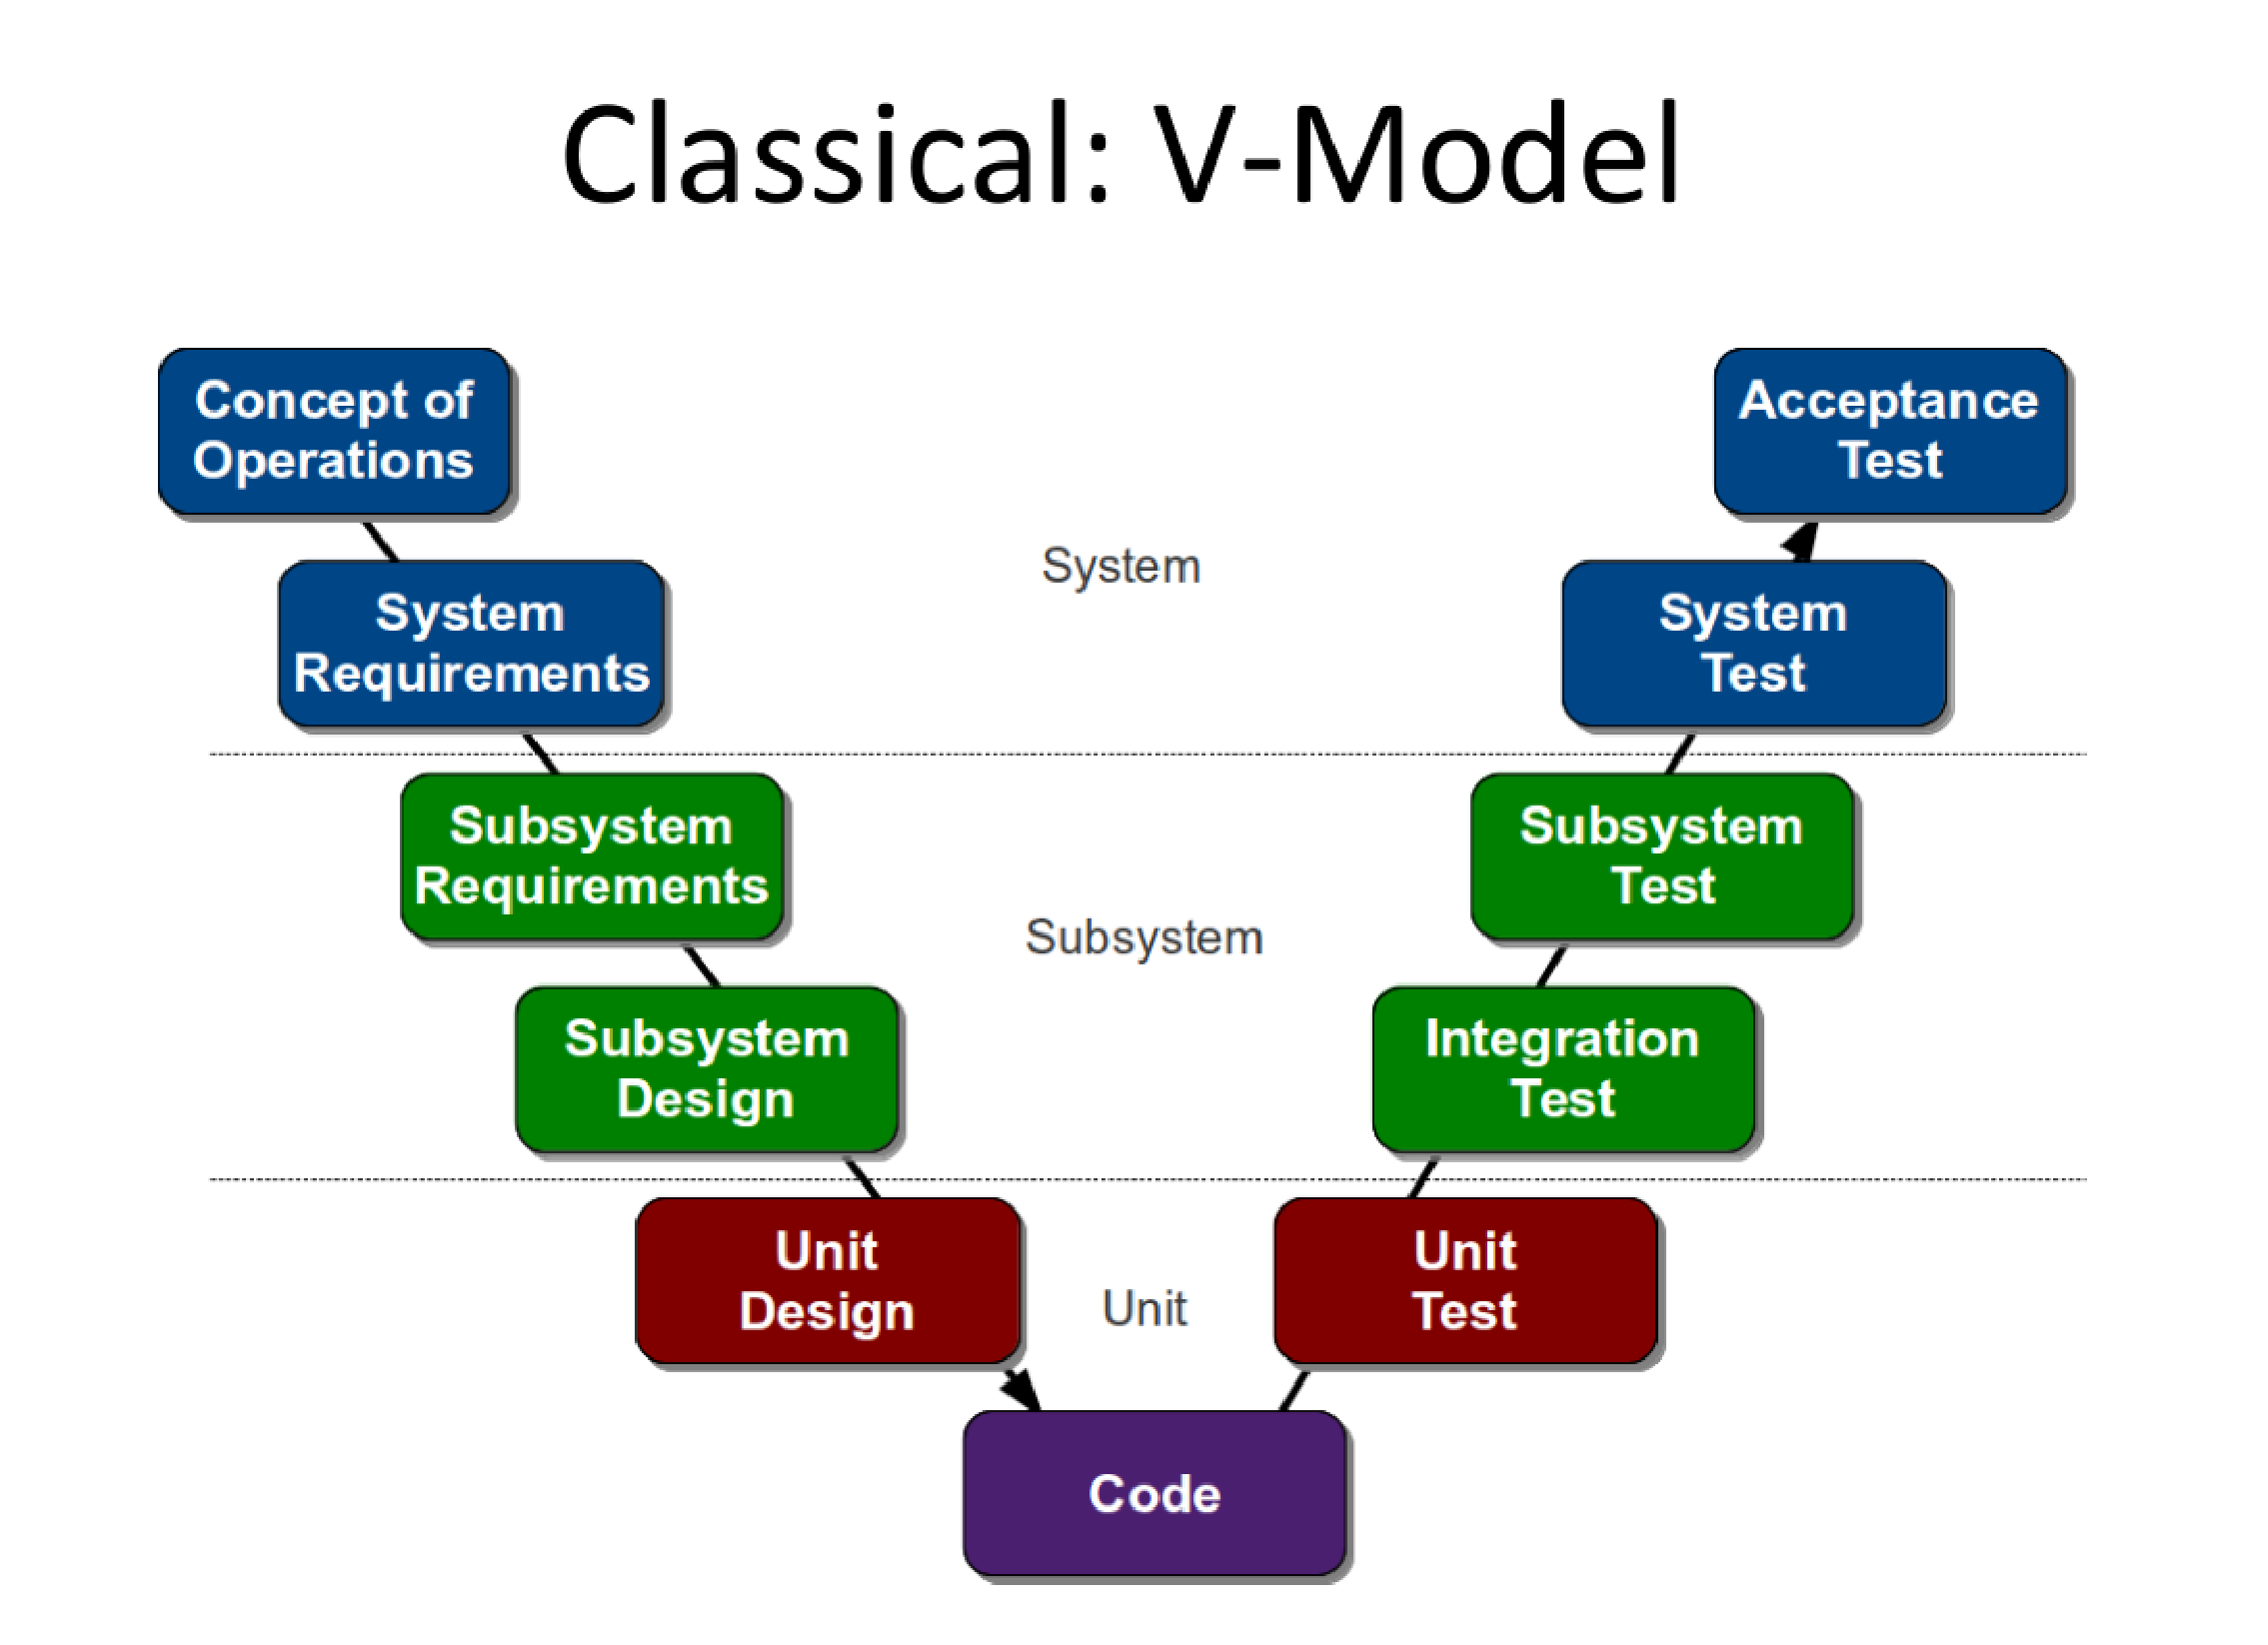
\includegraphics[scale=0.6,width = 15cm, height = 12cm]{images/VModel.pdf}
    \caption{A diagram showing the V model}
\end{center}
\end{figure}

\begin{figure}[h]
\begin{center} 
    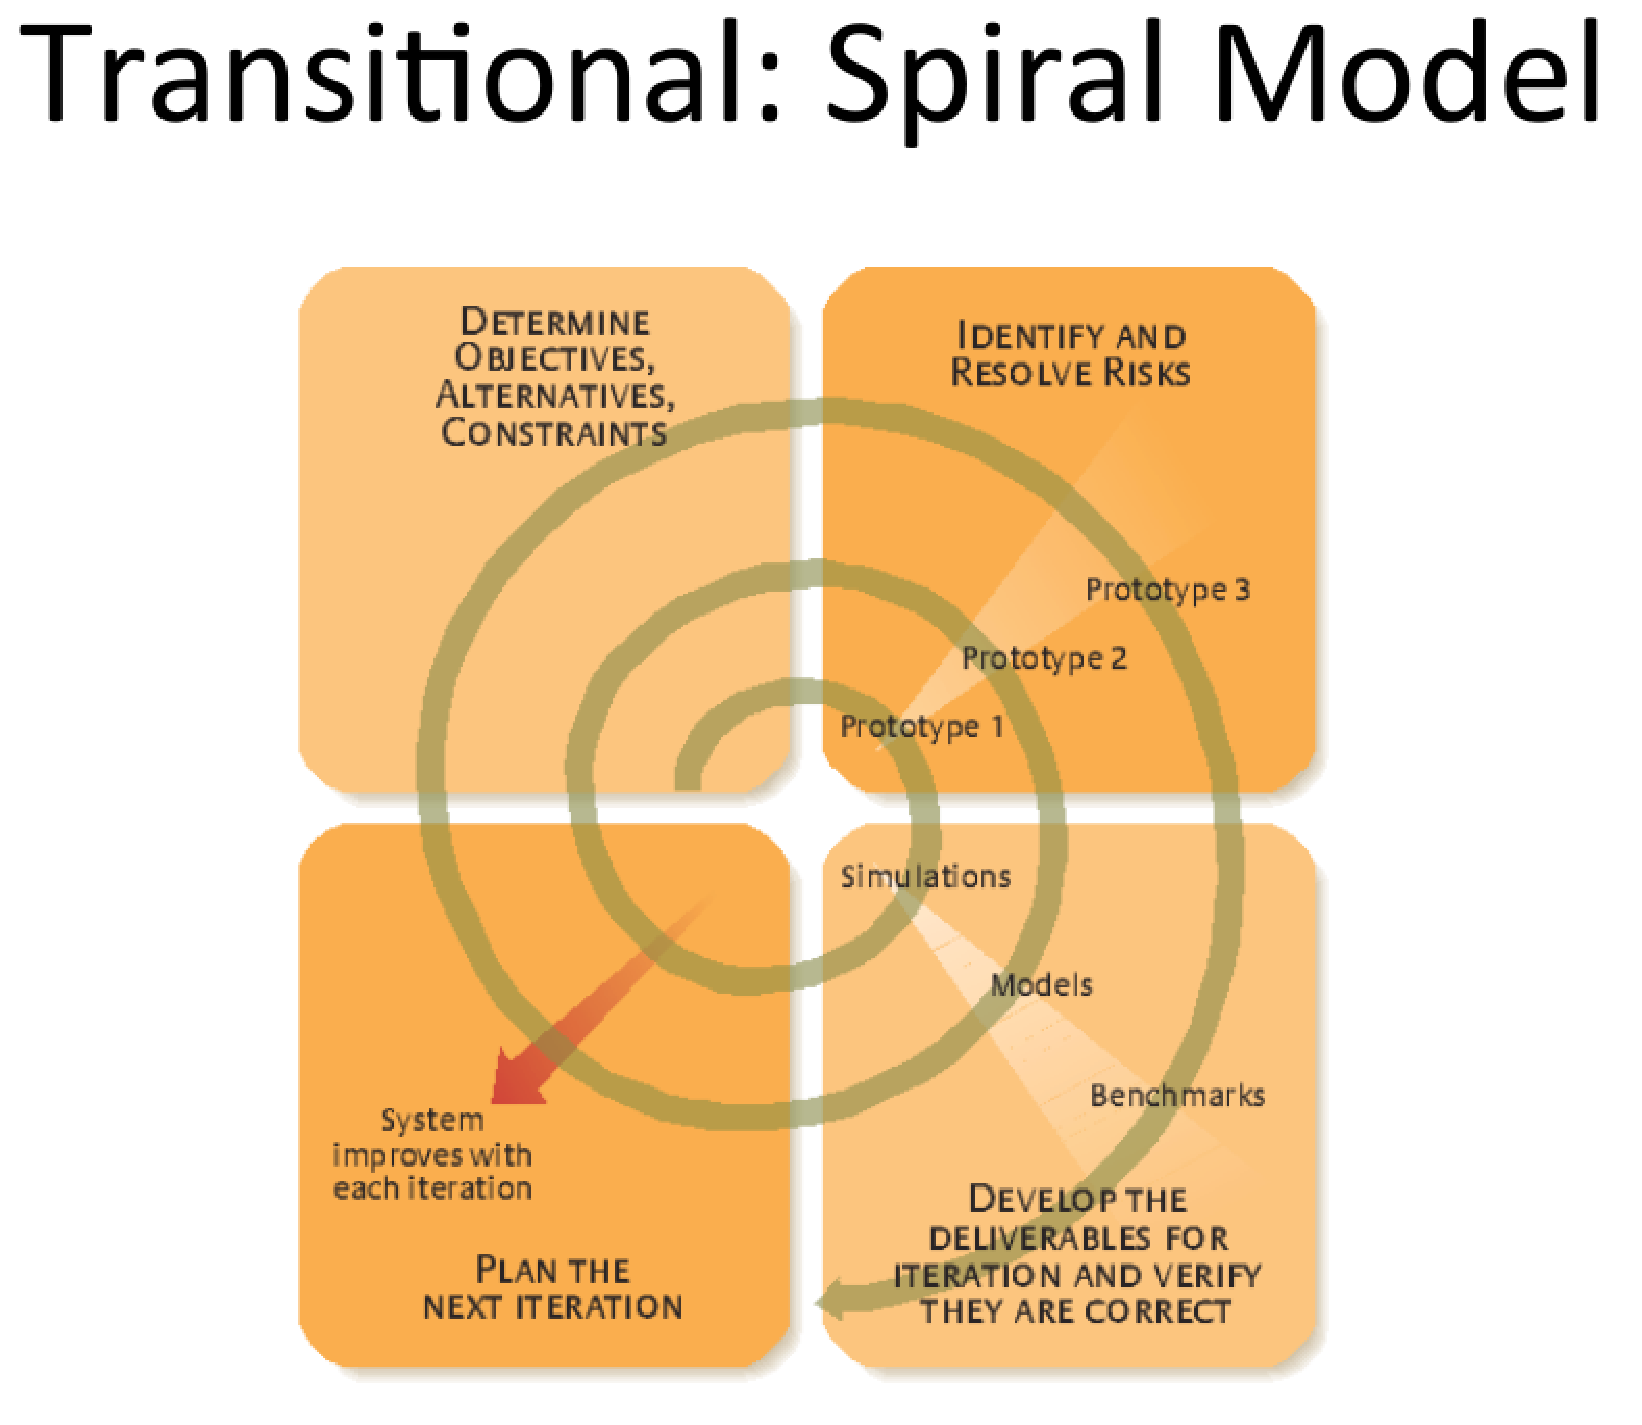
\includegraphics[scale=0.8,width = 15cm, height = 12cm]{images/Spiral.pdf}
    \caption{A diagram showing the spiral model}
\end{center}
\end{figure}

\begin{figure}[h]
\begin{center} 
    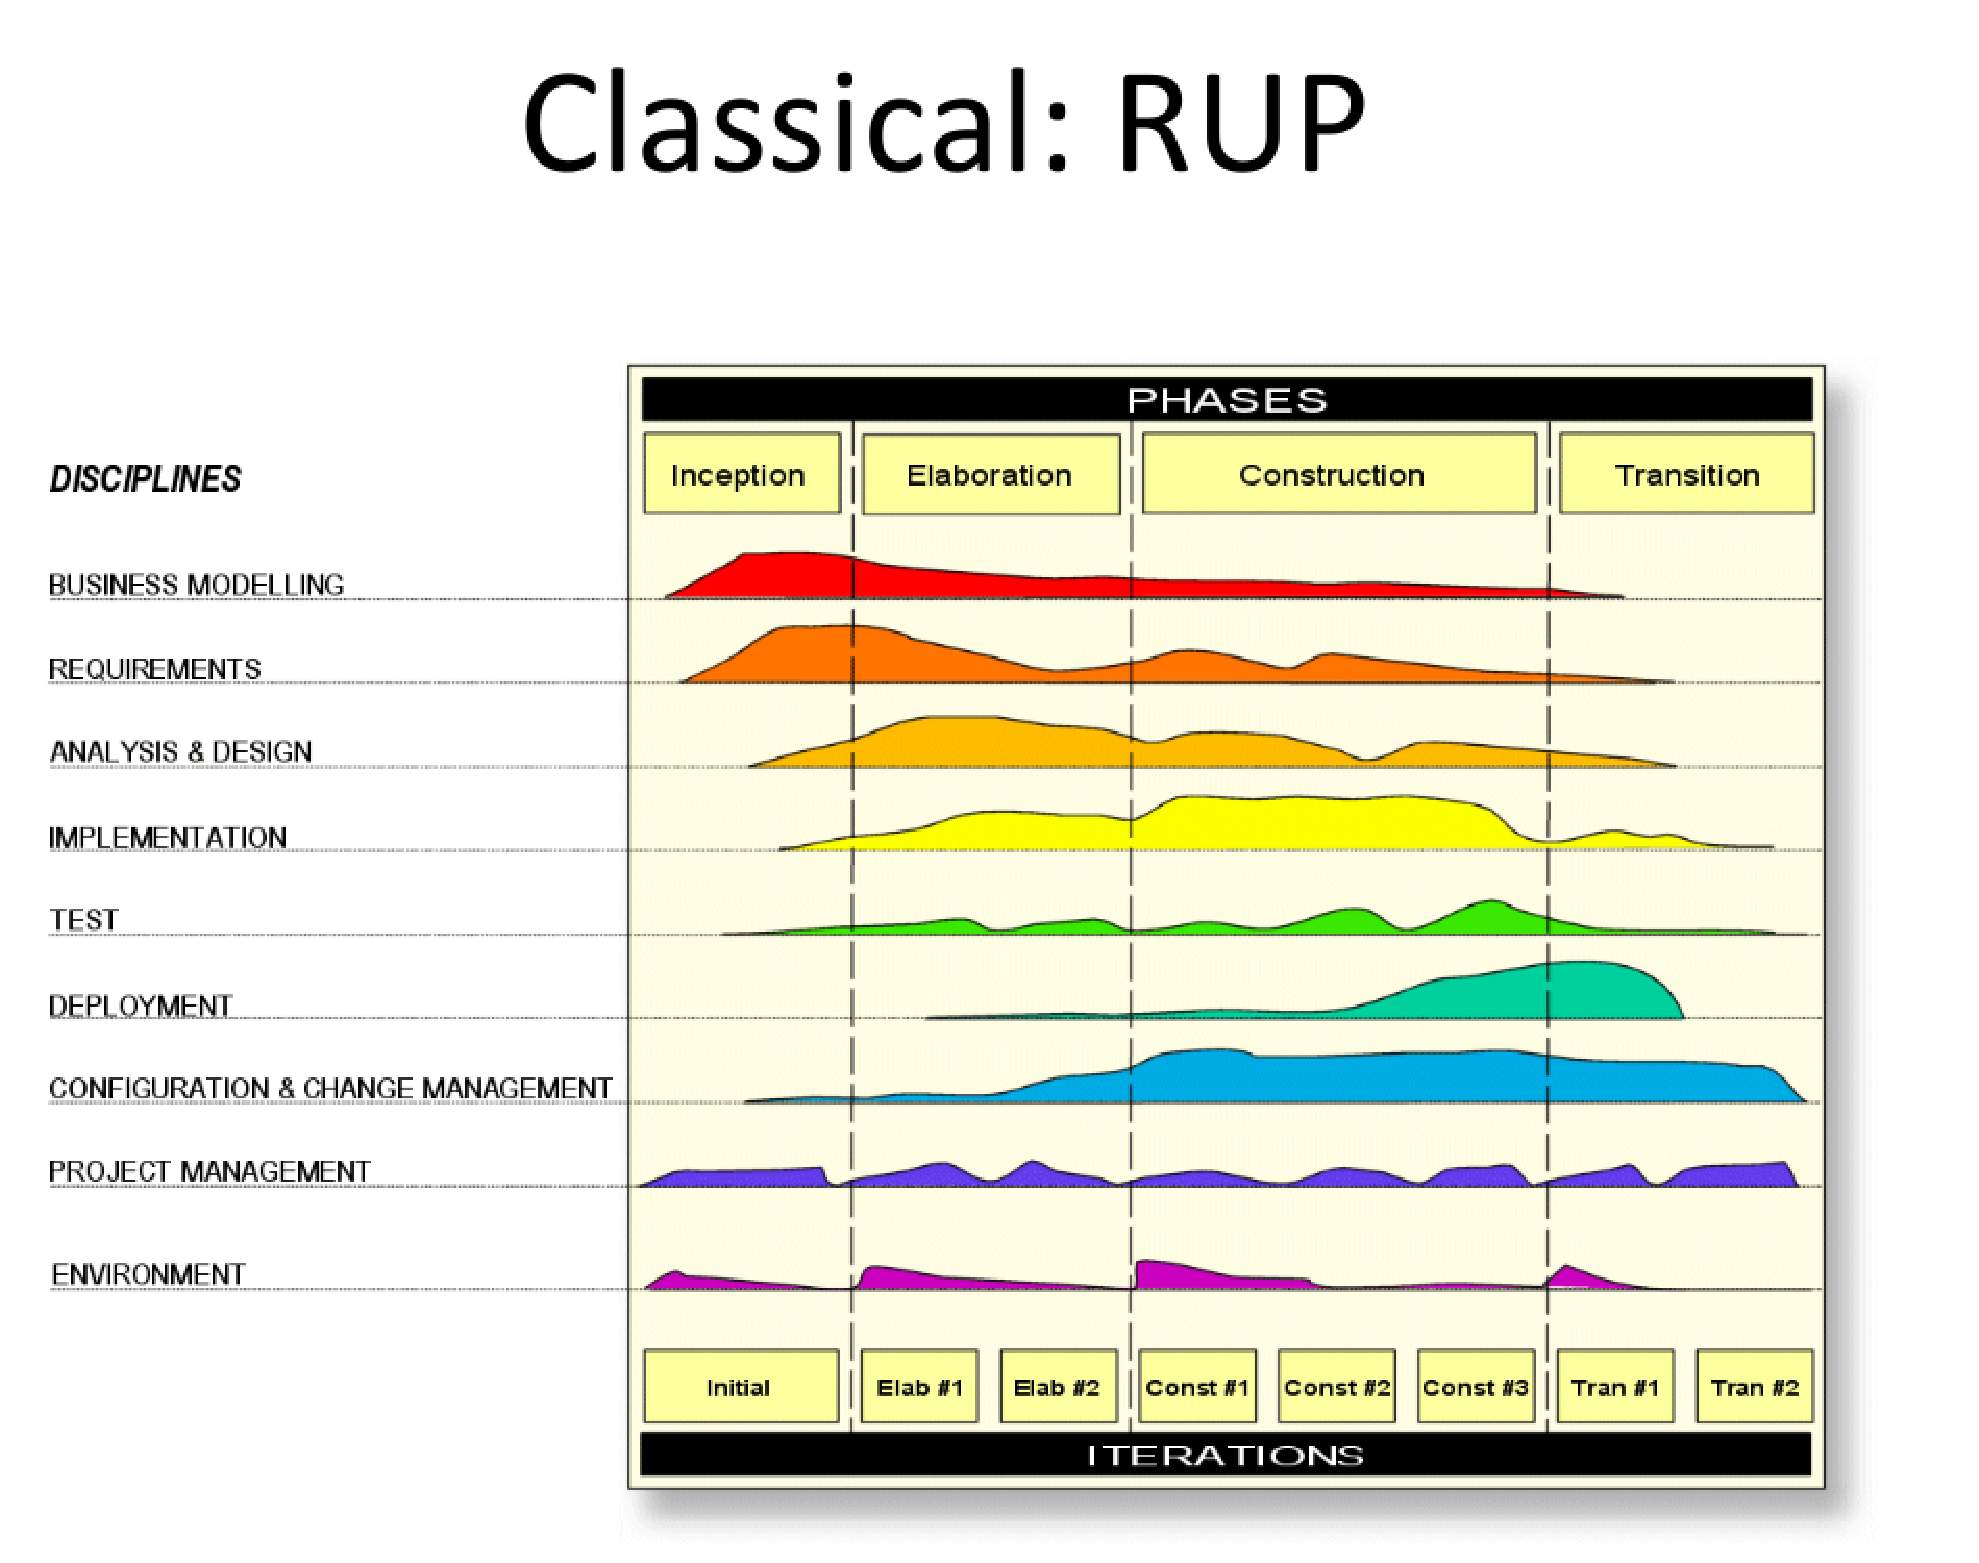
\includegraphics[scale=0.8,width = 15cm, height = 12cm]{images/RUP.pdf}
    \caption{A diagram of the RUP model}
\end{center}
\end{figure}

\textbf{Rational Unified Process(RUP) explained \newline} 
Rational Unified Process (RUP) establishes four phases of development, each of which is organized into a number of separate iterations that must satisfy defined criteria before the next phase is undertaken: in the inception phase, developers define the scope of the project and its business case; in the elaboration phase, developers analyze the project's needs in greater detail and define its architectural foundation; in the construction phase, developers create the application design and source code; and in the transition phase, developers deliver the system to users. 


\section{Agile Programming}
Agile Programming Practice:
\begin{itemize}
\item Test first programming
\item Refactoring
\item Continuous integration
\item Simple design
\item Pair programming
\item Common codebase
\item Coding standards
\item Open work area
\end{itemize}

Manifesto for Agile Software Development:
\begin{itemize}
\item Individuals and interactions over processes and tools.
\item Working software over comprehensive documentation.
\item Customer collaboration over contract negotiation.
\item Responding to change over following a plan.
\end{itemize}

The terms on the right are valued, but those on the left are valued more.

Scrum is an Agile framework for completing complex projects. Scrum originally was formalized for software development projects, but it works well for any complex, innovative scope of work. The possibilities are endless. The Scrum framework is deceptively simple:

\begin{itemize}
\item A product owner creates a prioritized wish list called a product backlog.
\item During sprint planning, the team pulls a small chunk from the top of that wish list, a sprint backlog, and decides how to implement those pieces.
\item The team has a certain amount of time — a sprint (usually two to four weeks) — to complete its work, but it meets each day to assess its progress (daily Scrum).
\item Along the way, the ScrumMaster keeps the team focused on its goal.
\item At the end of the sprint, the work should be potentially shippable: ready to hand to a customer, put on a store shelf, or show to a stakeholder.
\item The sprint ends with a sprint review and retrospective.
\item As the next sprint begins, the team chooses another chunk of the product backlog and begins working again
\end{itemize}

\section{Comparison of Agile versus Plan-Driven Approach}
The tables in the following images compare the agile to a plan-driven approach. 
\begin{figure}[h]
\begin{center} 
    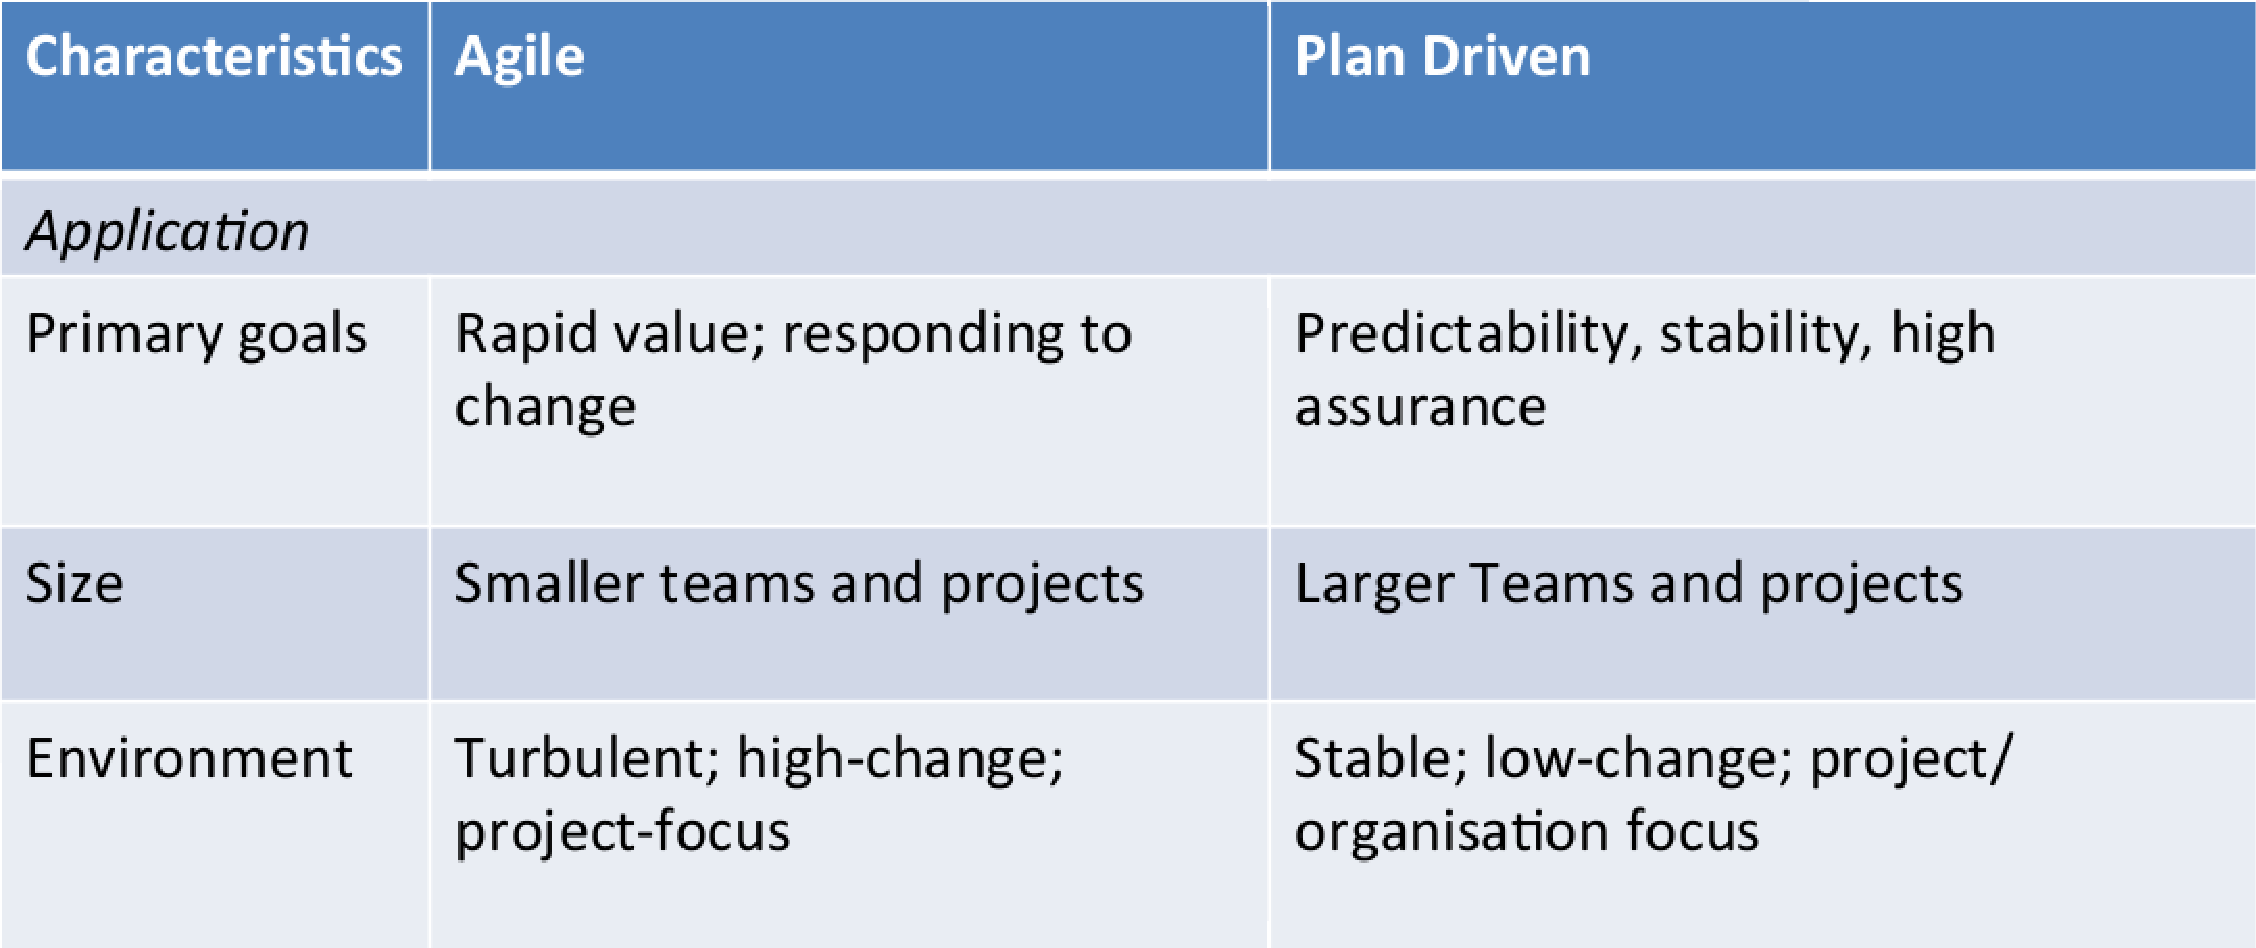
\includegraphics[scale=0.8,width = 15cm, height = 12cm]{images/AgileTable1.pdf}
\end{center}
\end{figure}

\begin{figure}[h]
\begin{center} 
    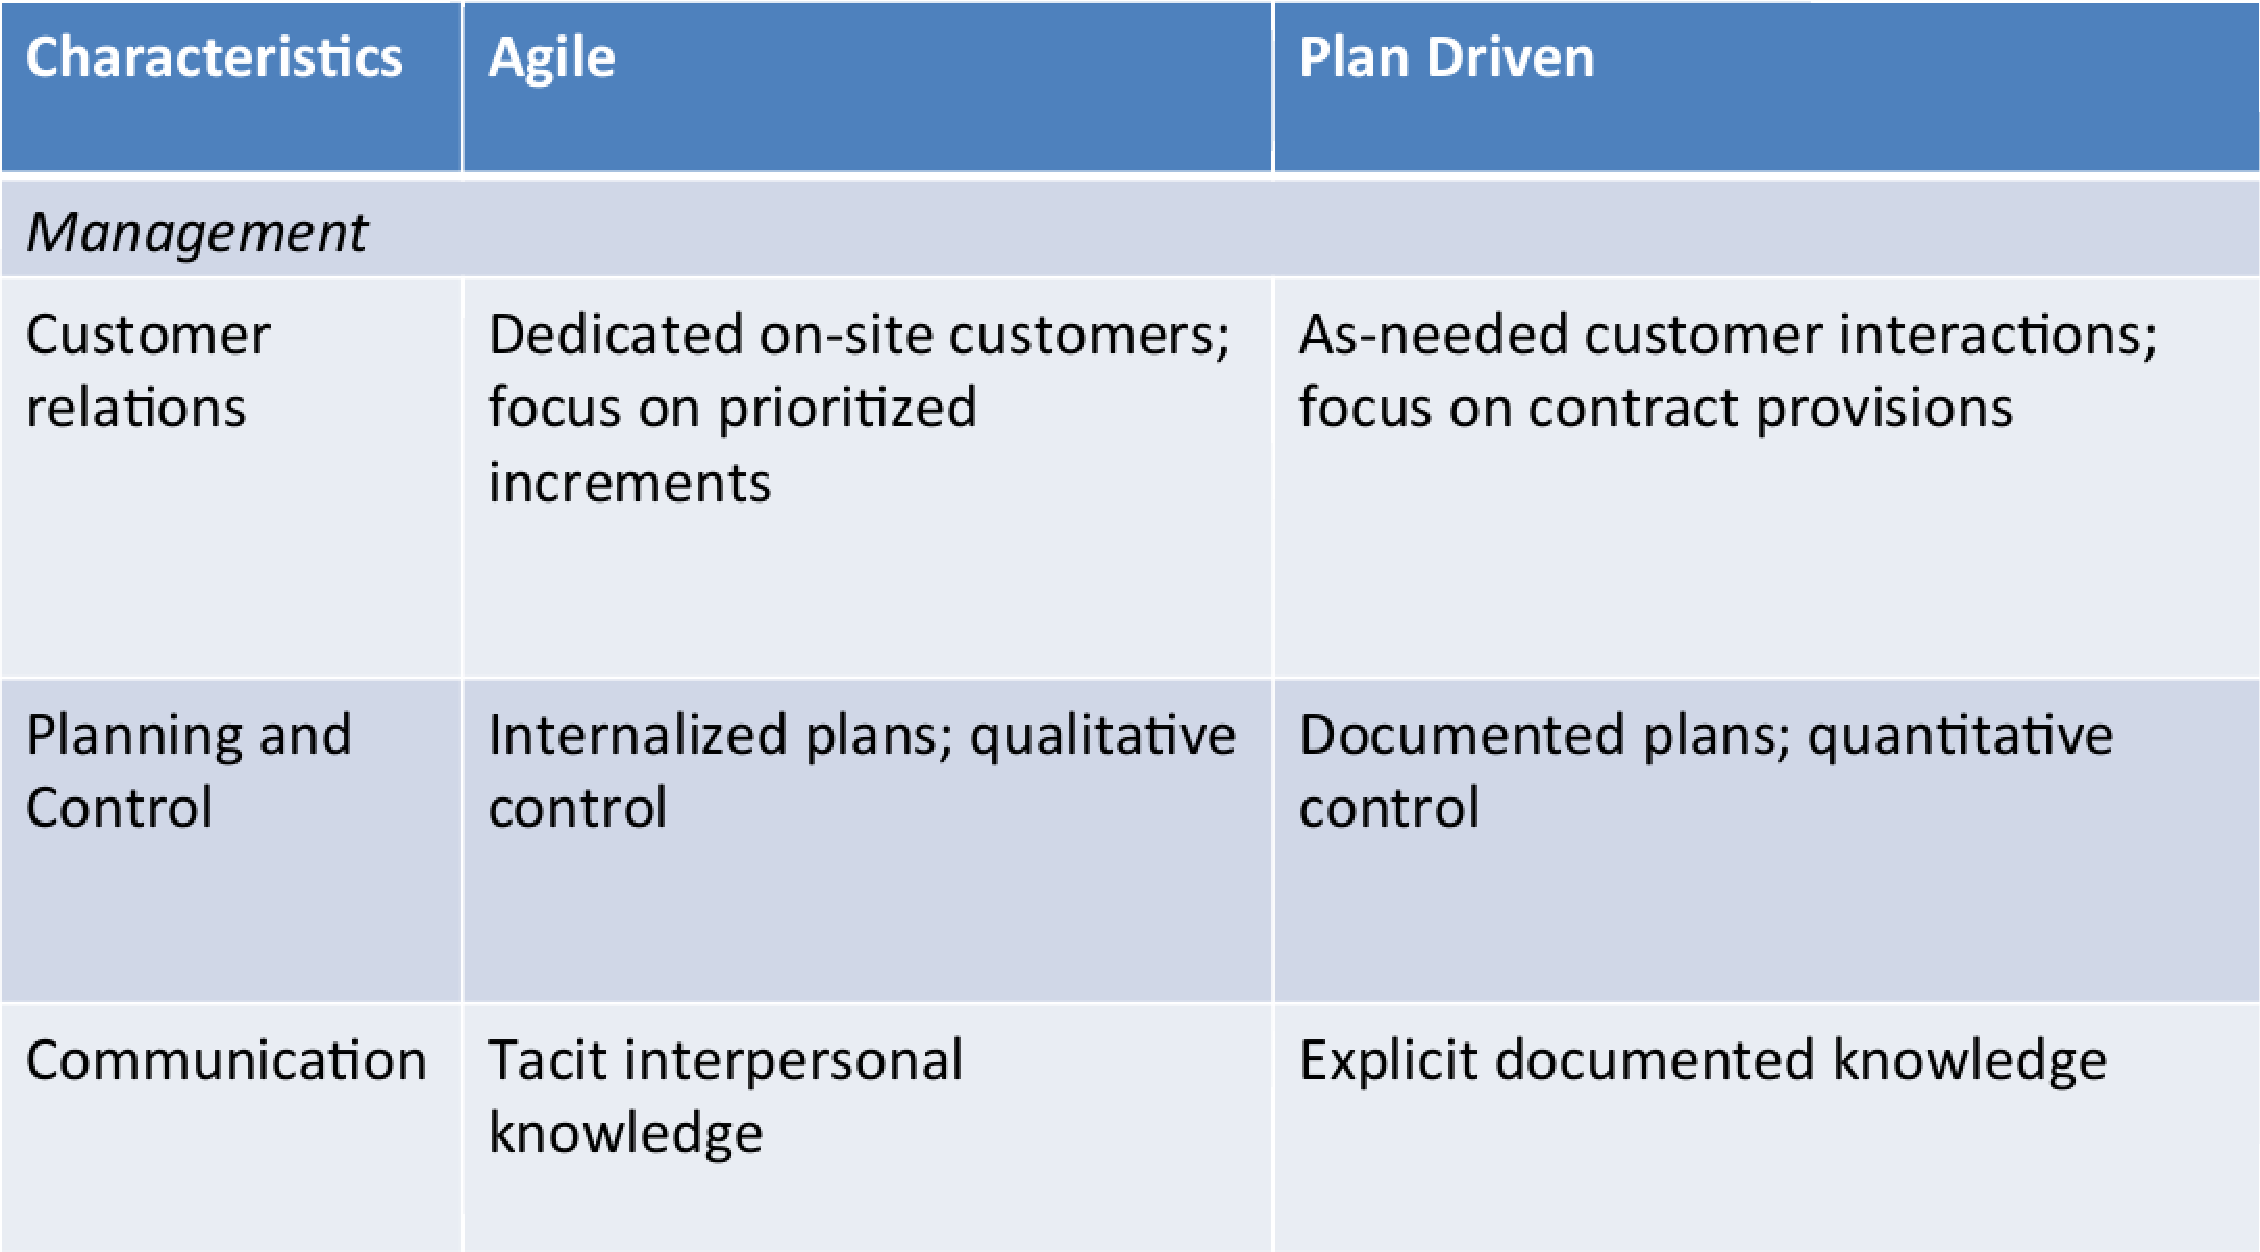
\includegraphics[scale=0.8,width = 15cm, height = 12cm]{images/AgileTable2.pdf}
\end{center}
\end{figure}

\begin{figure}[h]
\begin{center} 
    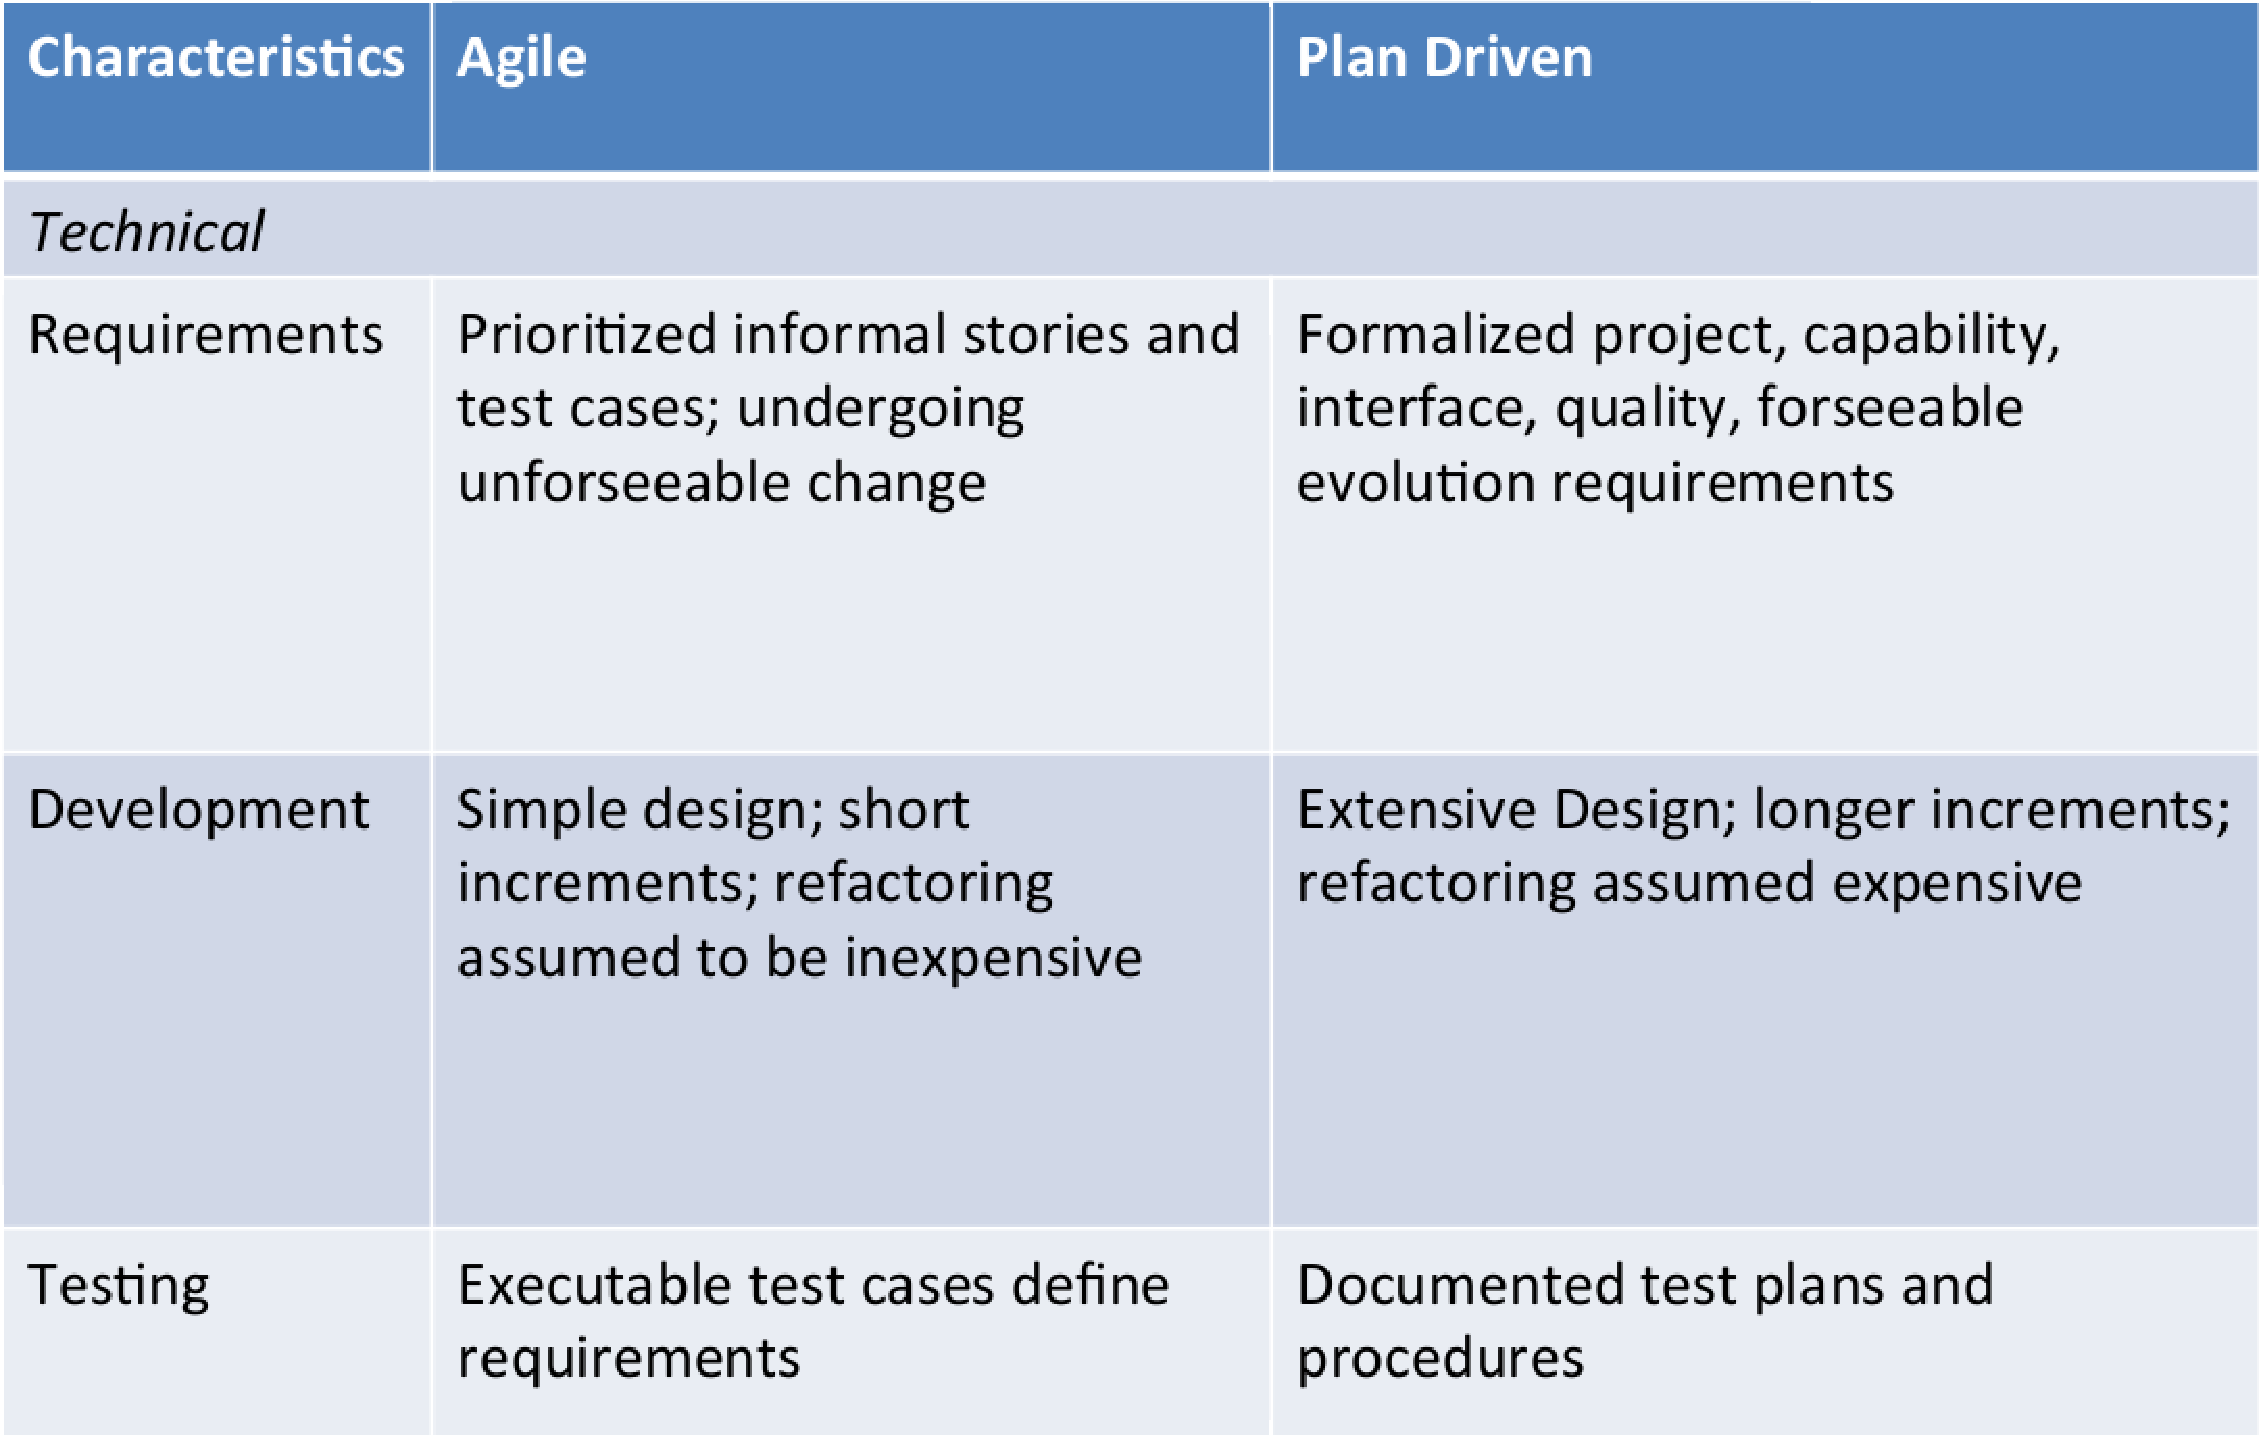
\includegraphics[scale=0.8,width = 15cm, height = 12cm]{images/AgileTable3.pdf}
\end{center}
\end{figure}

\begin{figure}[h]
\begin{center} 
    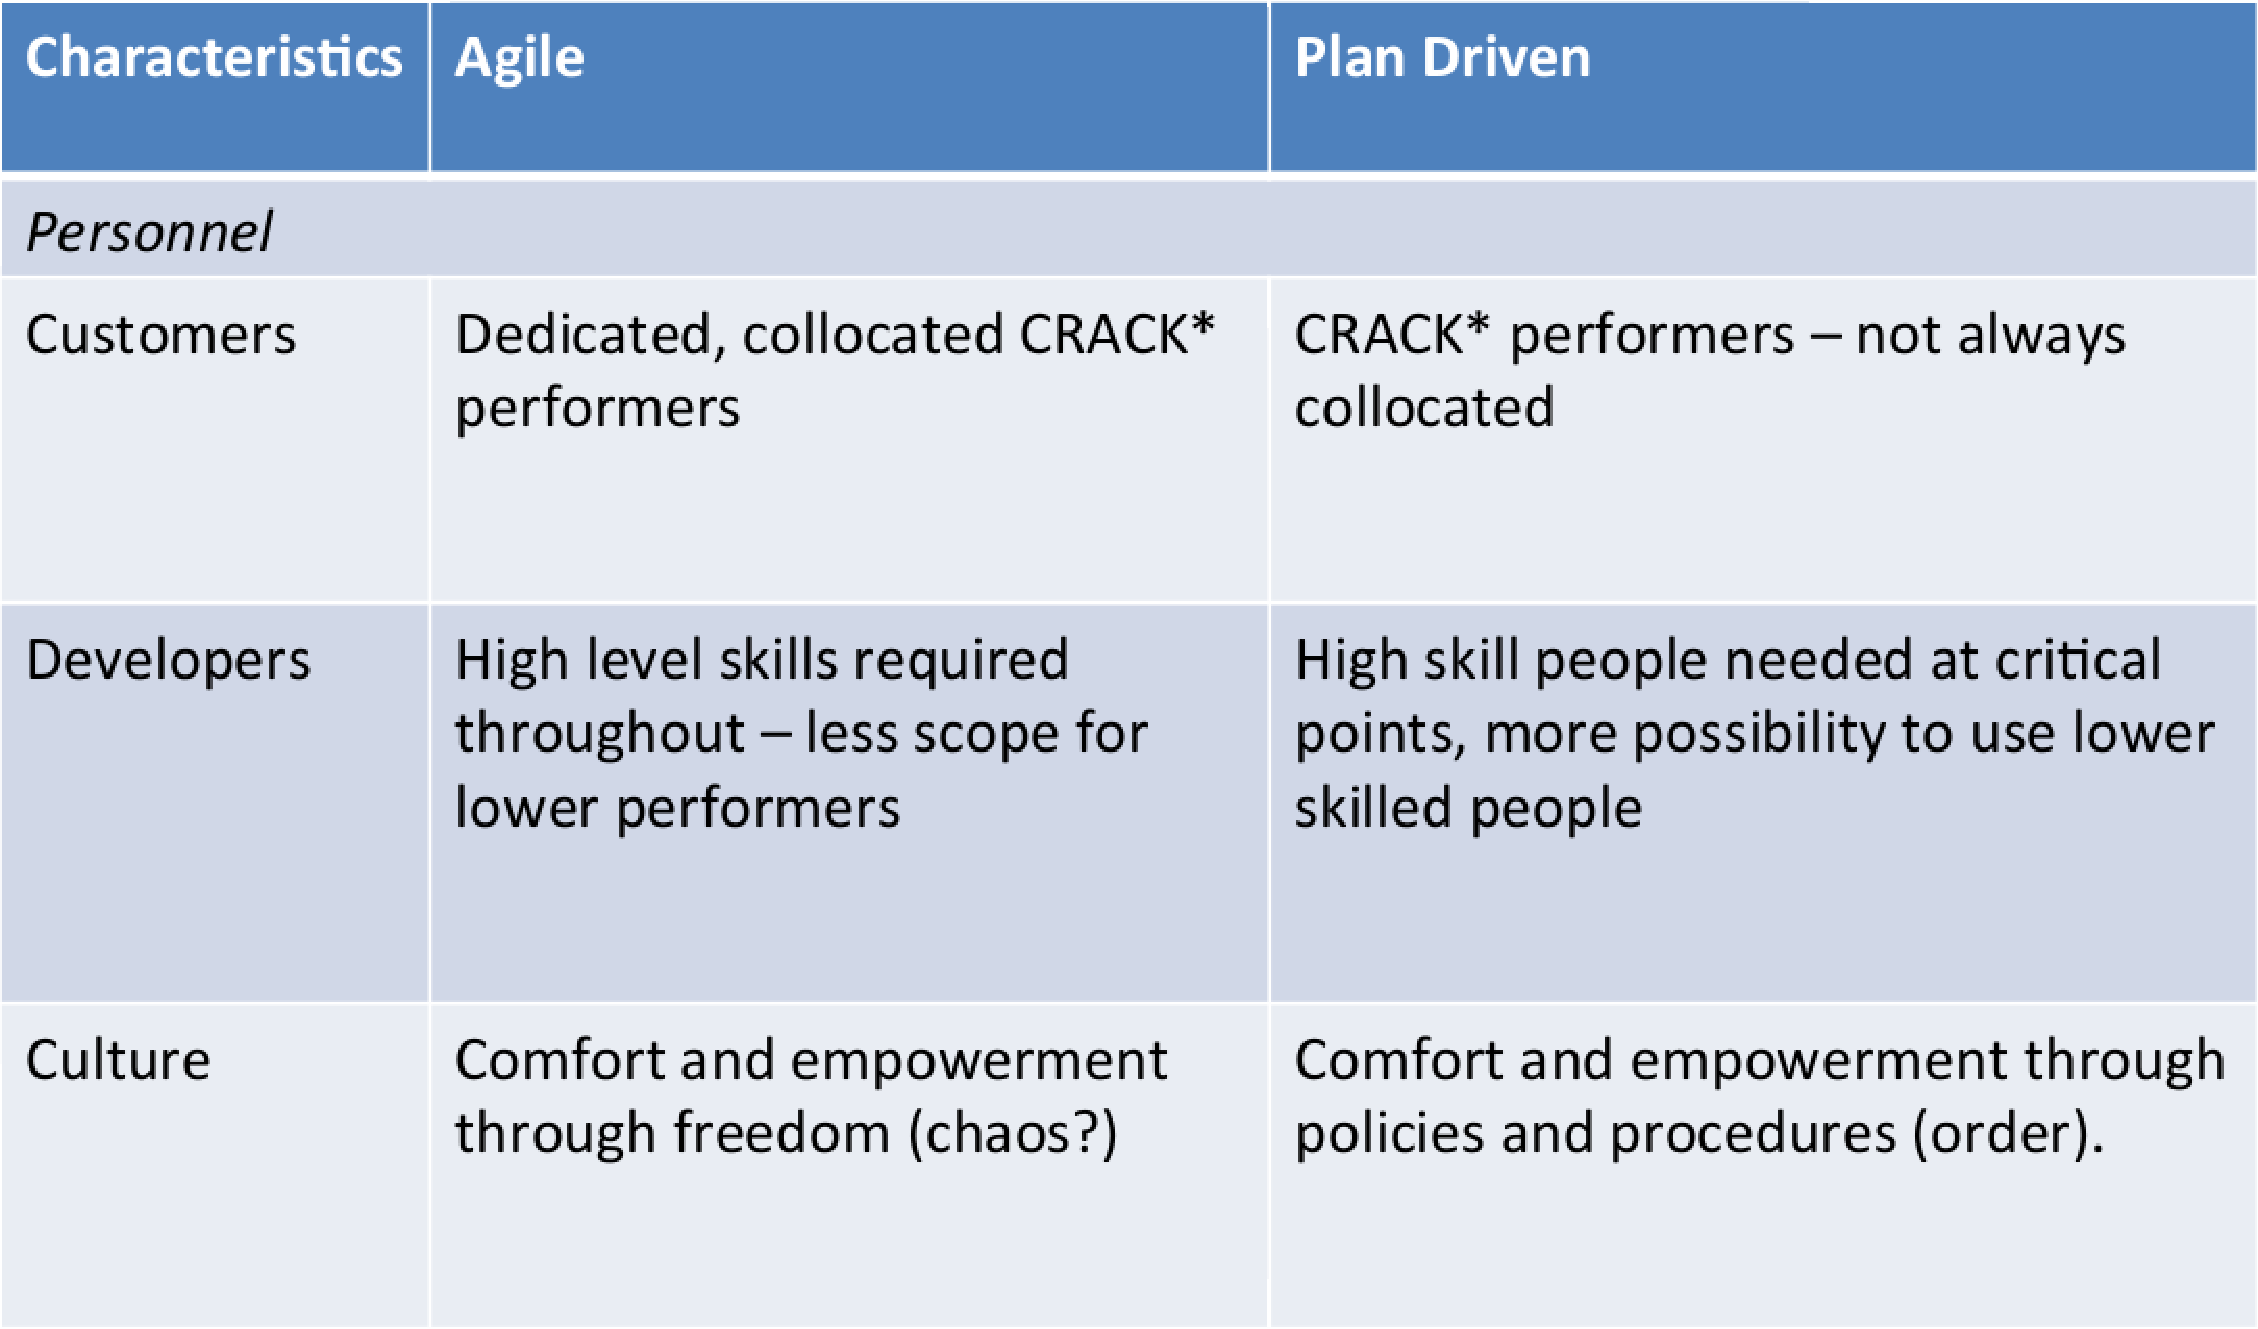
\includegraphics[scale=0.8,width = 15cm, height = 12cm]{images/AgileTable4.pdf}
\end{center}
\end{figure}

Key Points:
When developing software, work top-down and bottom-up at the same time – the balance of this depends on the size and complexity of the project.

General Rule:
As the size of the error/loss increases, the probability of the loss decreases. When the loss is small, the probability of it occurring is high. The relationship varies slightly depending on the project, but the general trend is as described above.

\begin{figure}[h]
\begin{center} 
    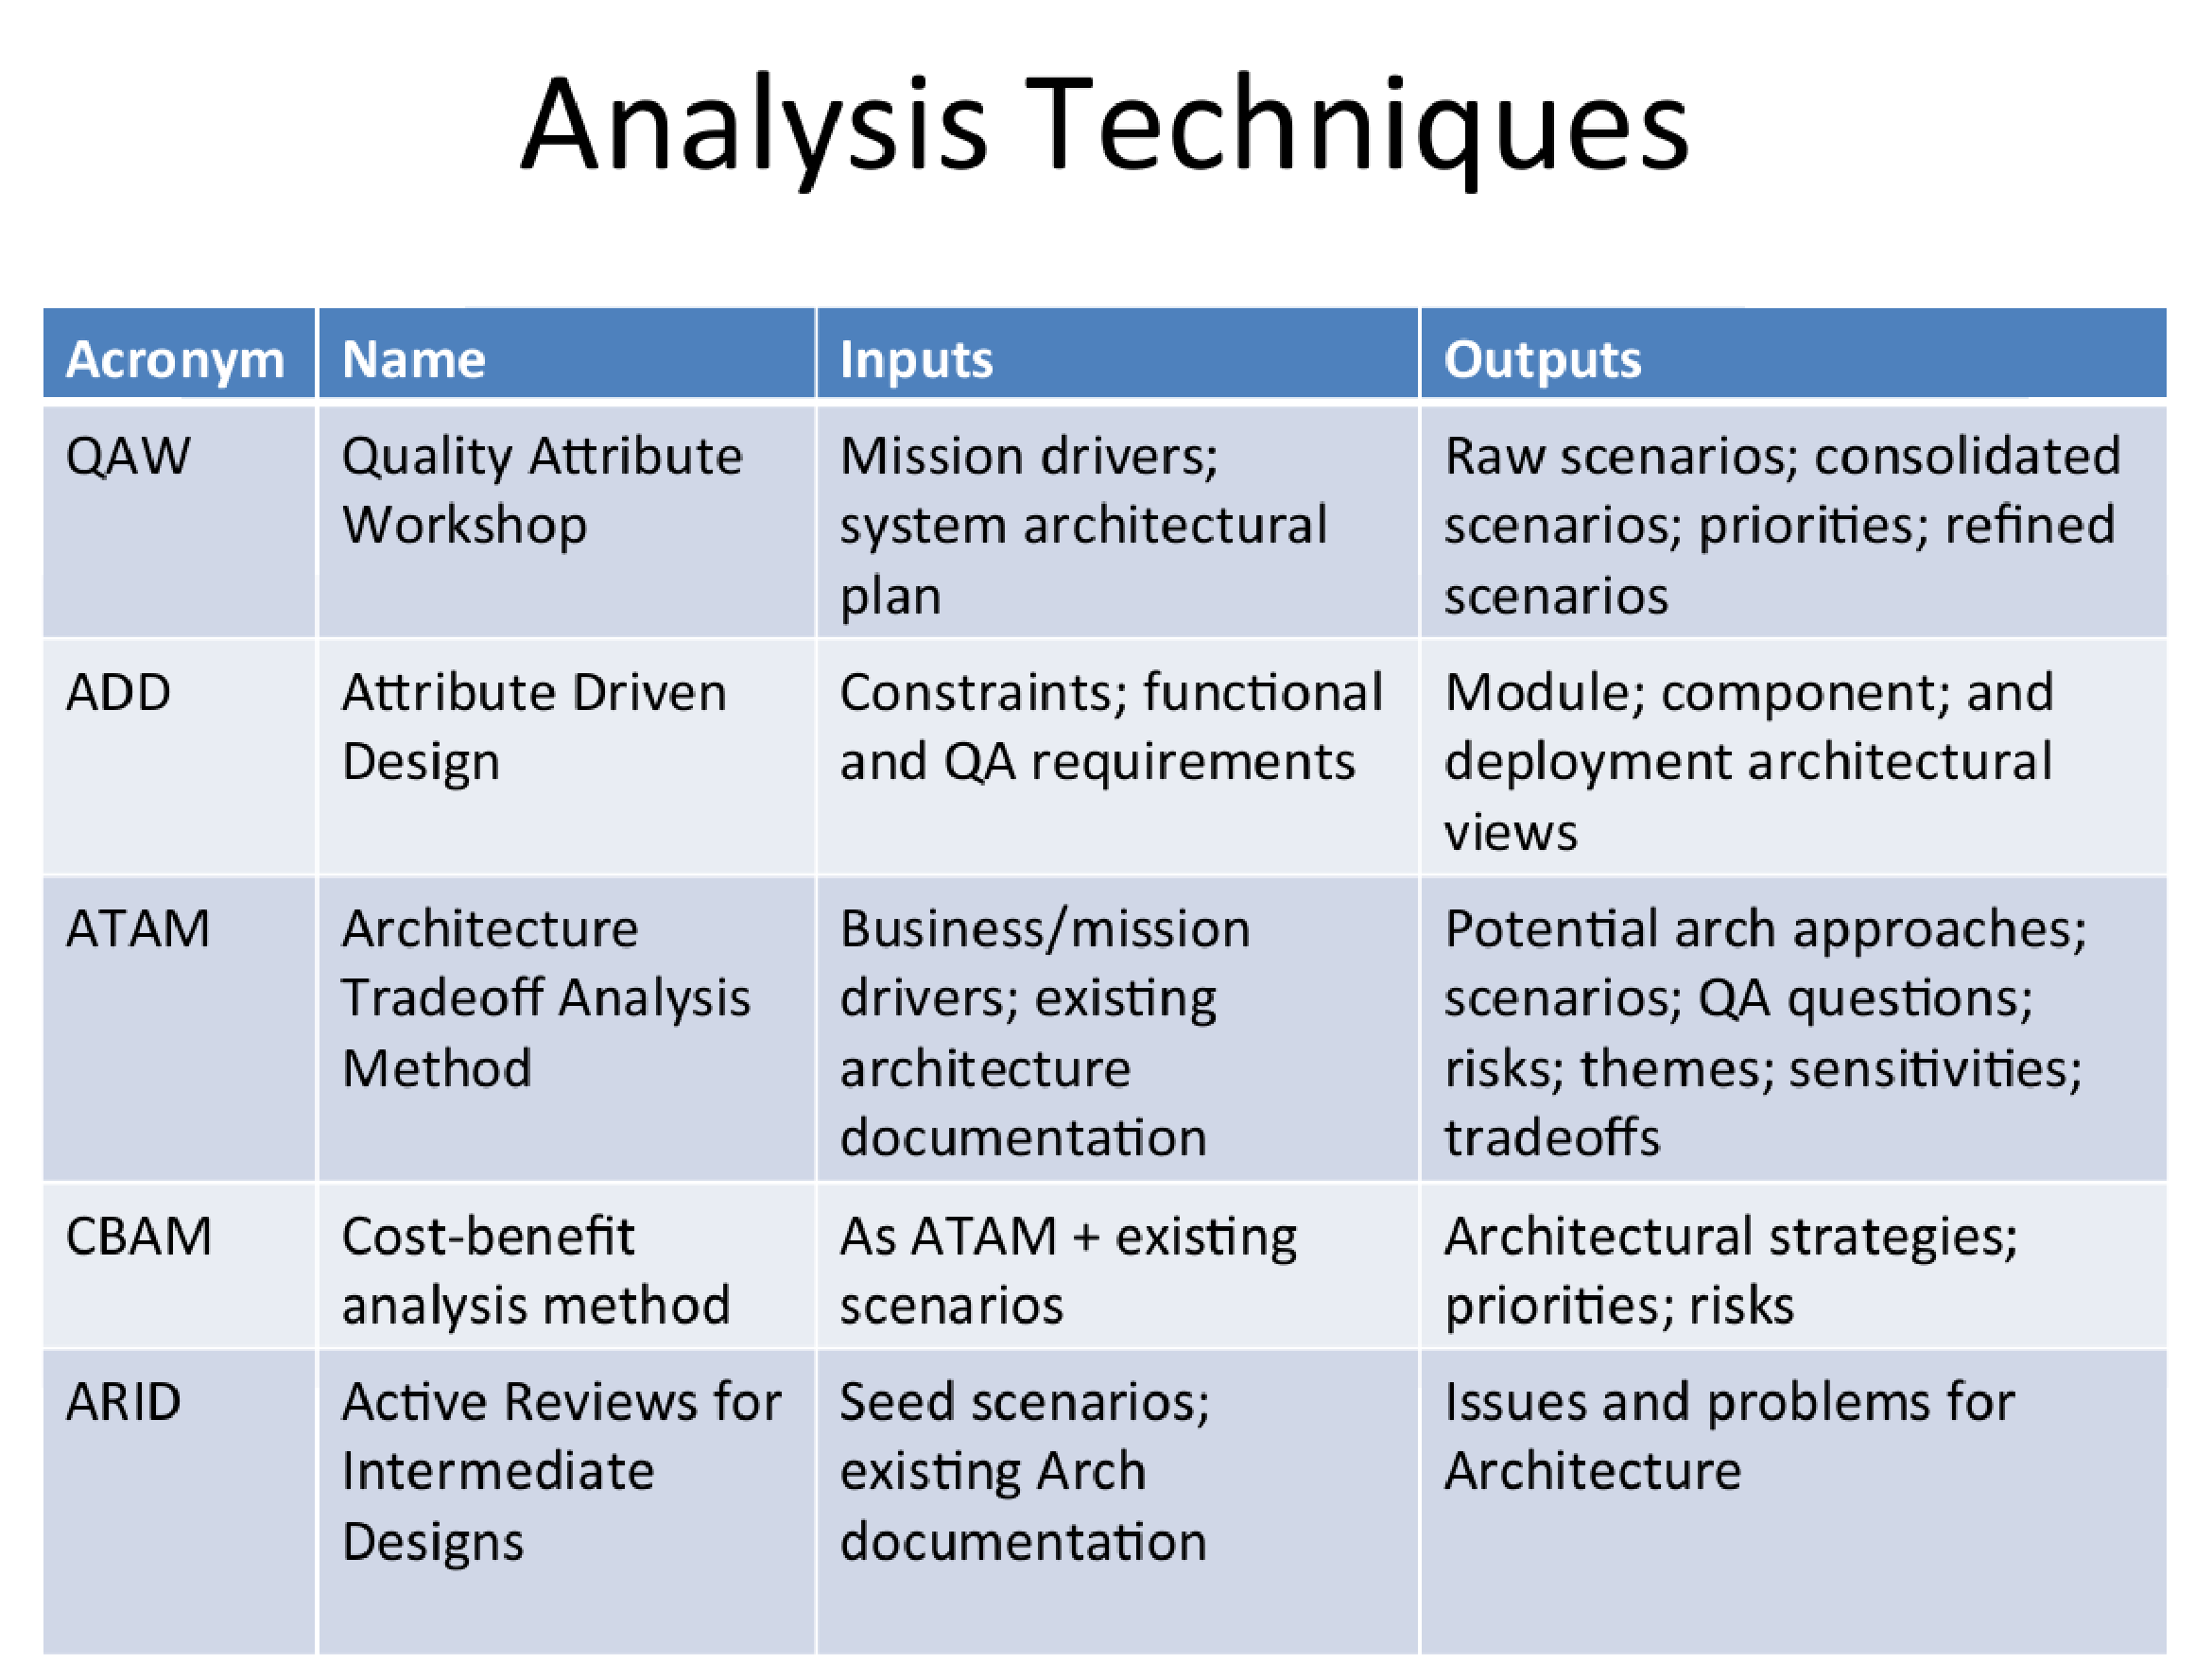
\includegraphics[scale=0.8,width = 15cm, height = 12cm]{images/Analysis1.pdf}
    \caption{Analysis Techniques}
\end{center}
\end{figure}

\begin{figure}[h]
\begin{center} 
    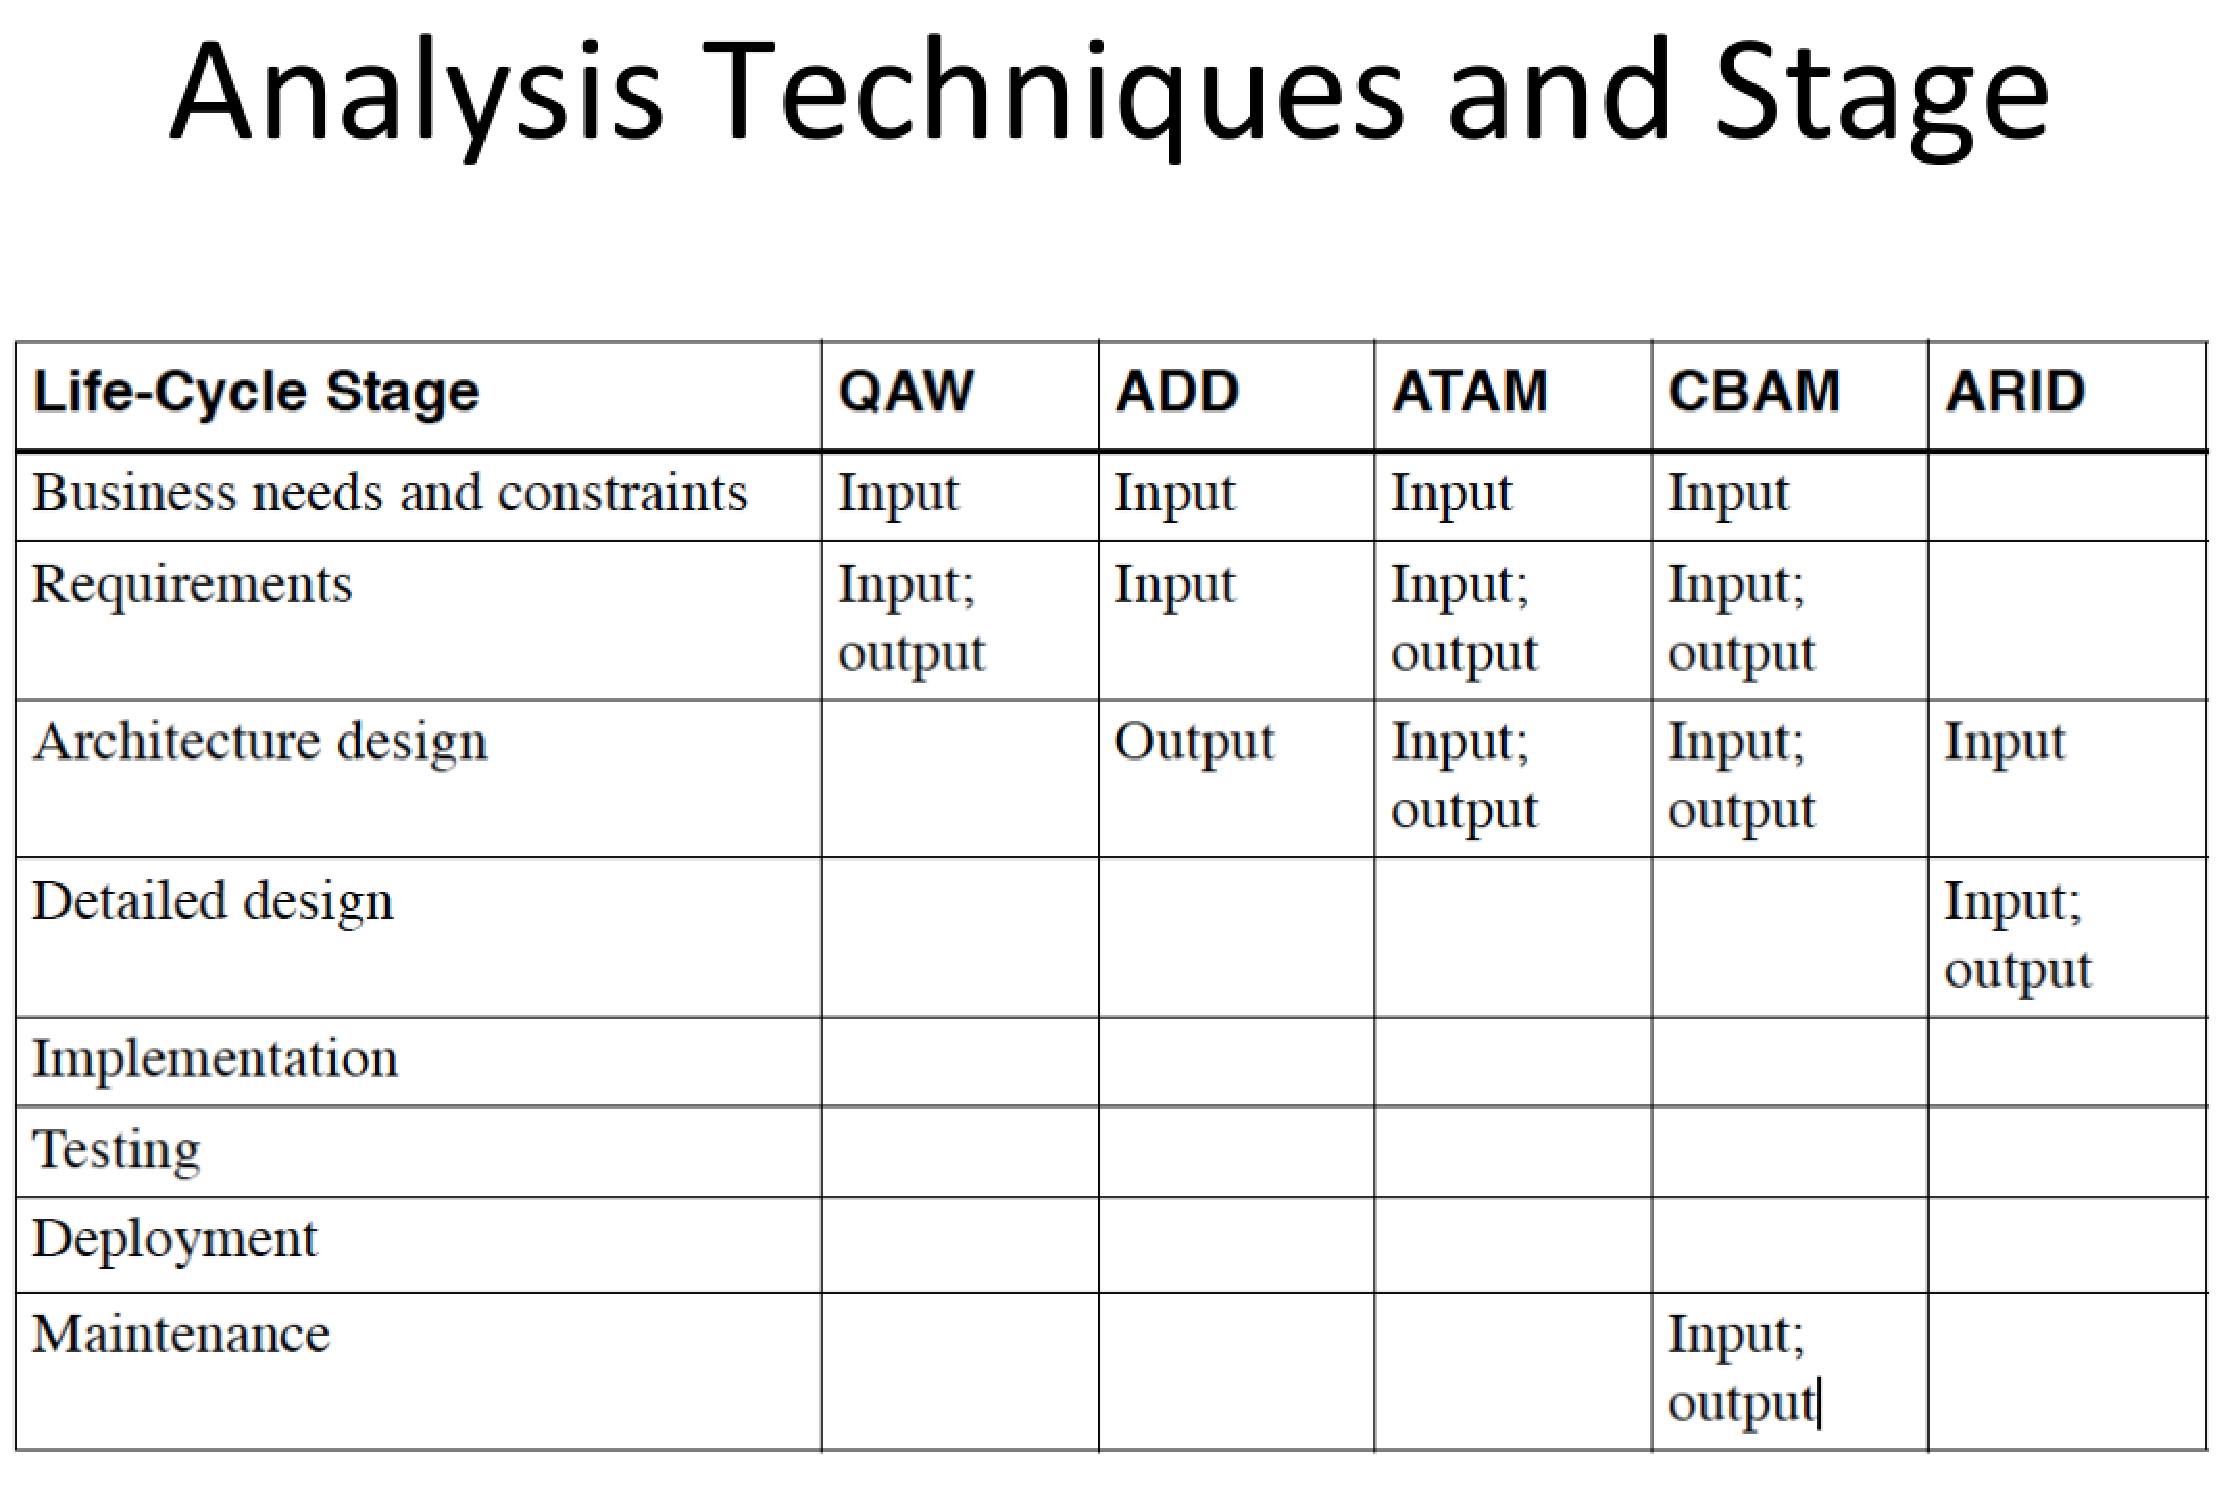
\includegraphics[scale=0.8,width = 15cm, height = 12cm]{images/Analysis2.pdf}
    \caption{Analysis Technique and Stage}
\end{center}
\end{figure}

\section{Summary}
\begin{itemize}
\item There are	many possible lifecycles and variants on	
these lifecycles.	
\item For any partcular	area of	actvity	we need to find the	
balance	between	agility	and	discipline.	
\item  Risk	links	discipline	and	agility	
\item QAs, scenarios and tactics help link architecture to	
more agile practice.	
\item Architectural	analysis techniques	provide	useful	
information for lifecycle activities, however they are	
arranged in	a process.	
\item Processes	like the Spiral	Model or ICM provide	
processes that are	sensitive to project risk.
\end{itemize}

\chapter{Product Line Architecture}
\section{Overview}
Software often comes in families. Thus, it makes sense to try to share components. Many real-world products are produced in a product line – such as cras, for example.

A software product line is a collection of software-intensive systems that share a common, managed set of features that are developed from a set of core assets in a prescribed way. 

Think of different, successive versions of the same product released by a company – they are all based on the same baseline architecture. When the number of products in it increase beyond a certain number, it starts to become profitable for the company using this technique.

\section{Key Properties}
Key properties of this product line architecture:
\begin{itemize}
\item usually are directed by the business goals in the application domain
\item all products share a software product line architecture
\item new products are all structured by this product line architecture and are built from services and components
\item product lines spread costs over several products
\item Architecture must be flexible enough to support variation in the products
\item Software components – general enough to support variability
\item All other components of the software must be general enough to deal with variation
\item People need to be skilled in architecture and product lines
\end{itemize}

\section{Benefits to organization}
There are several benefits to the organization:
\begin{itemize}
\item much better productivity
\item quicker delivery time to the market – so maintain market presence and sustain growth
\item enable mass customization
\item improve product quality
\item better predictability of cost, schedule, and quality
\end{itemize}

\section{Main Terms}
\textbf{Core Asset Development:} improving the base components in terms of qualities, products they support, and architecture

\textbf{Product Development:} identifying and building products to meet market need inside the product line

\textbf{Management:} monitoring and improving the processes, tools, and practices

\section{Different Techniques in Introducing Product Lines}
\begin{itemize}
\item Proactive – up front investment to develop the core assets
\item Reactive – start with one or two products and use them to generate core assets – so see how well they do and then “react”
\item Incremental – develop core assets as the business need evolves
\end{itemize}
The general process involves considering the business strategy, consequences for products, consequences for processes and methods, and consequences for tools and the organization.

\section{Pros of Using a Product Line:}
\begin{itemize}
\item Increased competitiveness on the market because of reduced hardware resource consumption and reduced time to market for new features
\item Development efficiency – reuse, easy configuration of software products, increased planning accuracy
\item Quality  - interface integrity, reuse of core assets
\item Customer needs – differentiation by individual software solutions, clear feature-cost mapping
\end{itemize}

\section{Architectural Features of Product Lines:}
\begin{itemize}
\item Control of resource consumption, such as memory
\item Good interface management
\item Layers provide the opportunity to share applications without knowing the details of some components
\item Software is reusable so that component redesign is easy and quick
\item Standardization is important
\item Important to standardize and develop tools that ease interchange between the company and it clients (toolchains)
\end{itemize}

\section{Phased Introduction}
This is how a company would start applying a software product line (called phased introduction) :
\begin{itemize}
\item Investigate and customize product line engineering
\item Design and apply adequate processes and methods
\item Roll out and institutionalize the standard development process
\end{itemize}

\chapter{DevOps}
\section{Overview}
This is the process of seeing development and operations as a unified entity. It oversees the whole process and all stages of developing software. It is the set of practices intended to reduce the time between communicating a change to a system and the change being placed into normal operation while ensuring necessary quality. 

The Whole Application Lifecycle:
1)  Define - ideation
2)  Develop - idea to working software
3)  Operate - working software in production, value realization
4)  Measure - actionable learning

\section{OSLC}
OSLC standards simplify lifecycle integration, which leads to cost savings and increased flexibility.
It is the foundational technology for all integration, and is the natural choice for standardizing loosely-coupled integrations in new domains. 

\begin{figure}[h]
\begin{center} 
    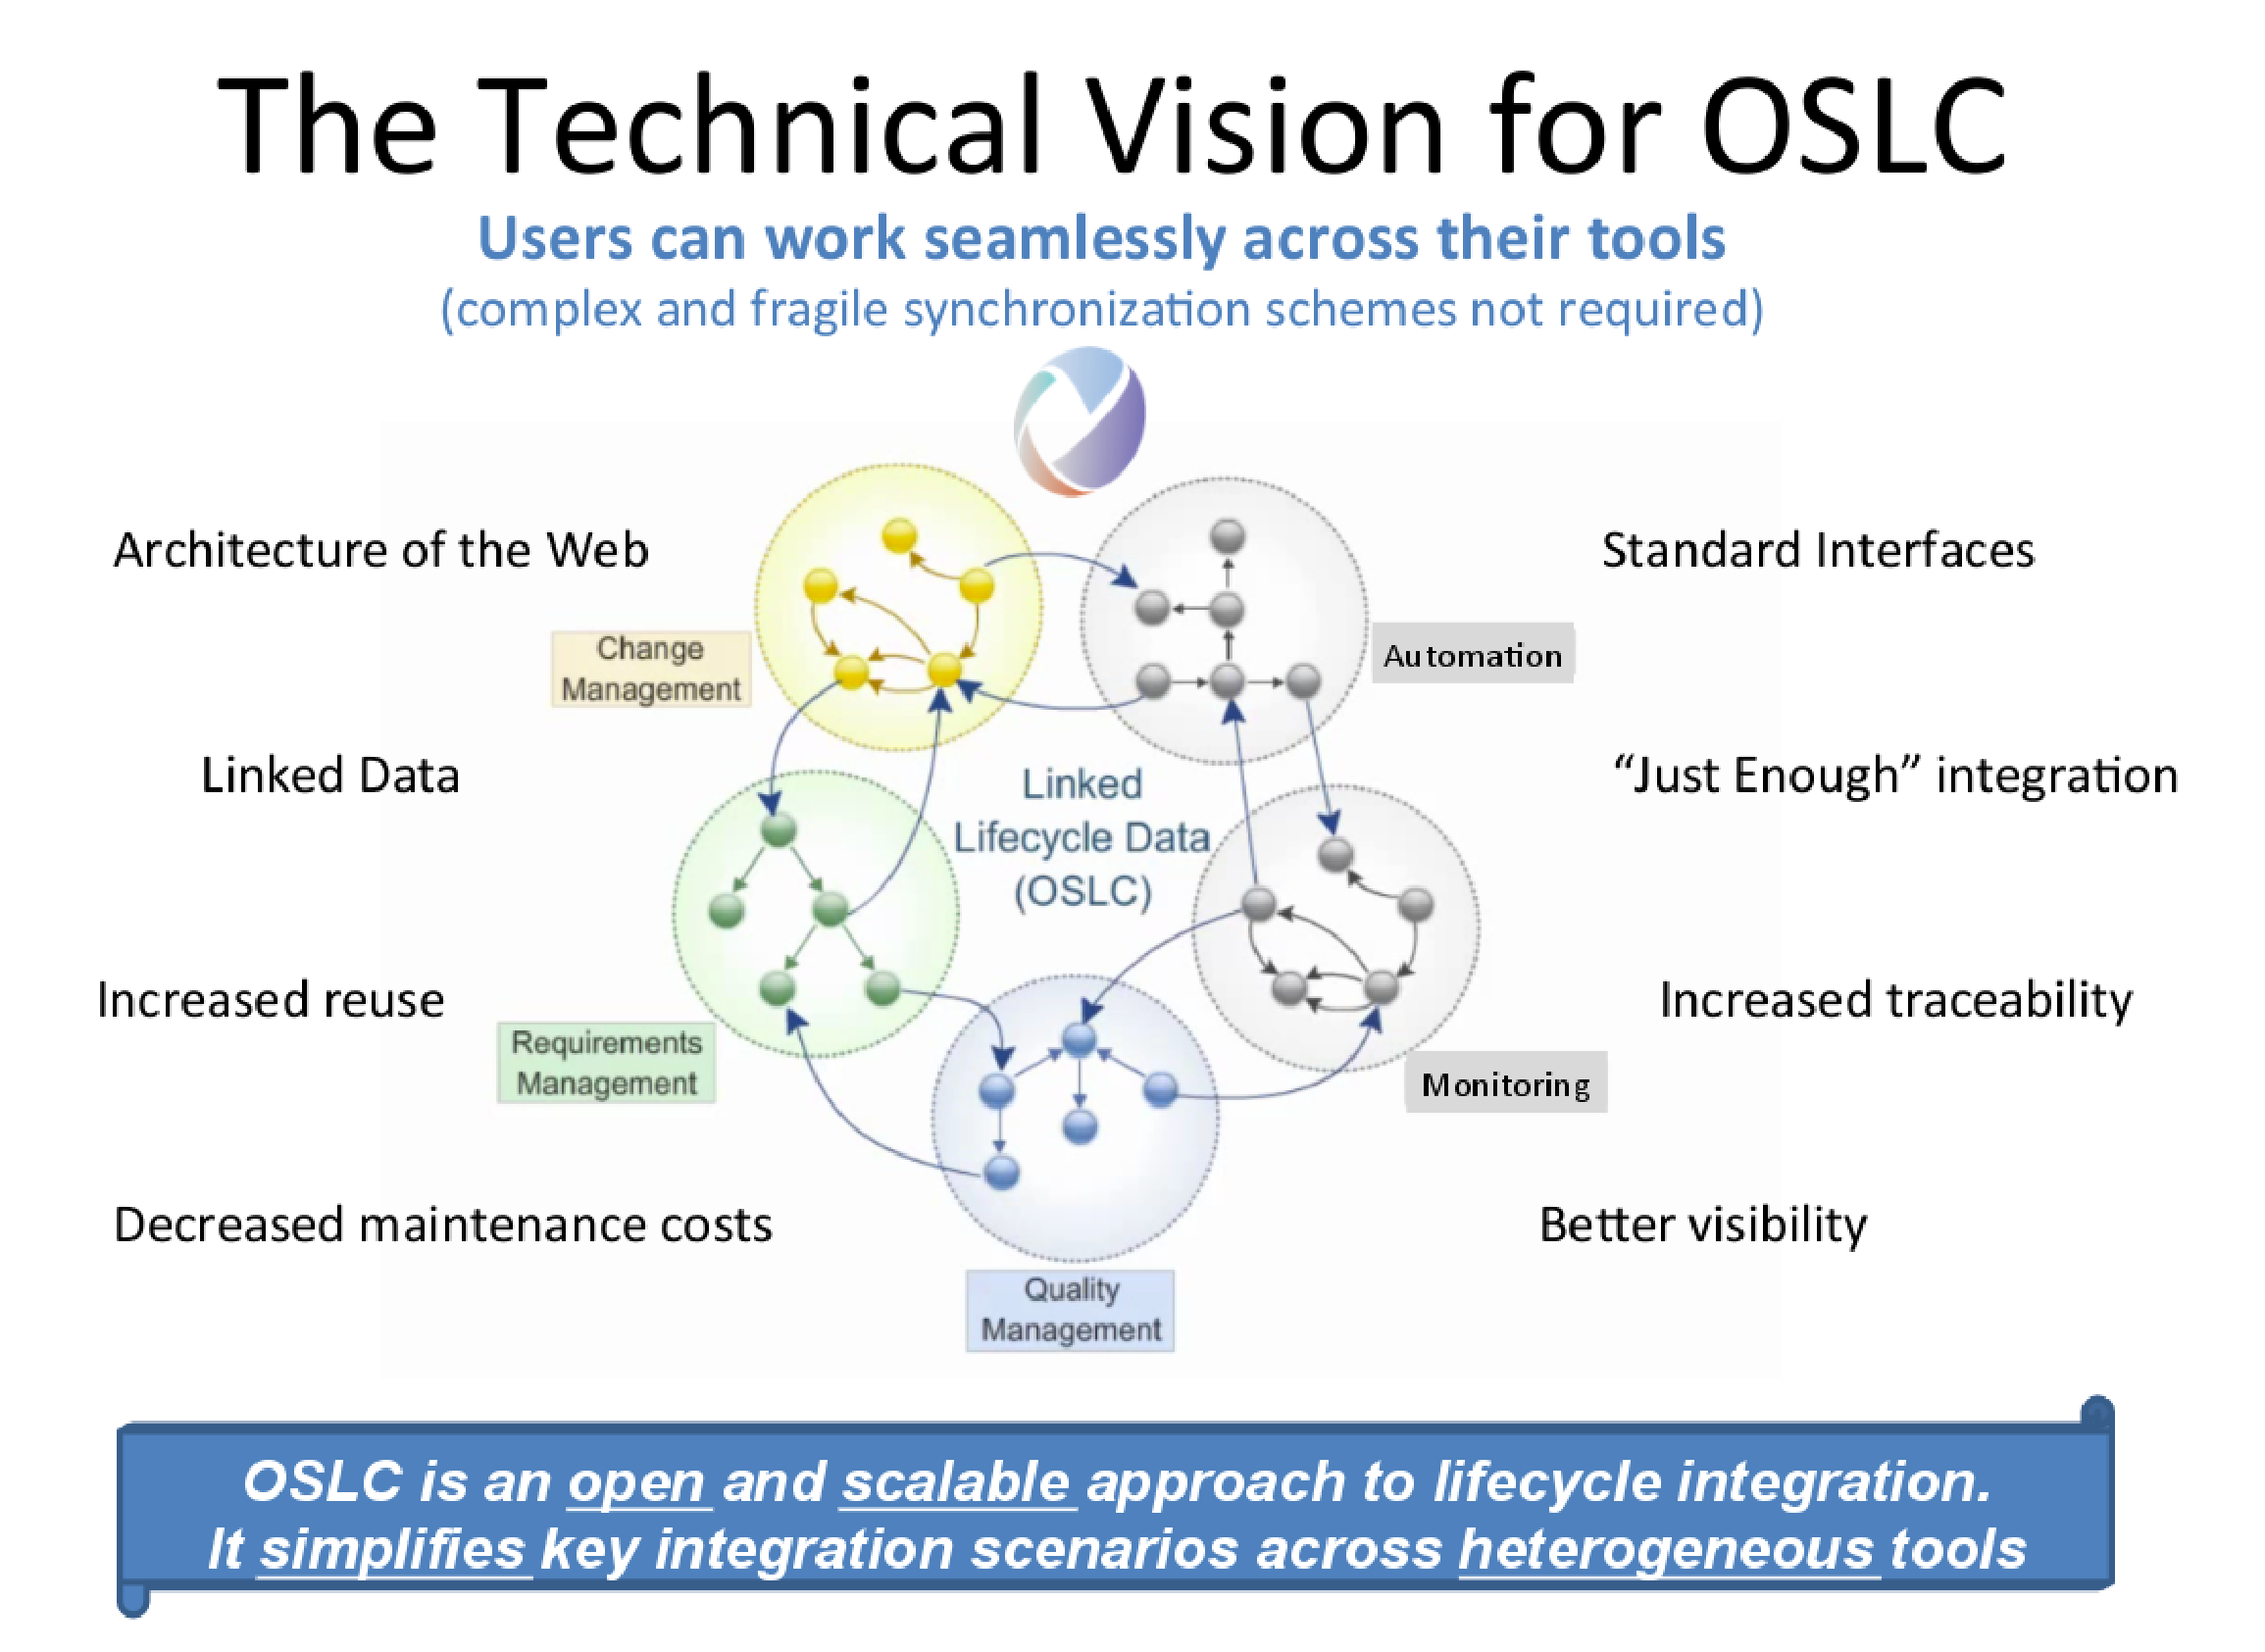
\includegraphics[scale=0.8,width = 15cm, height = 12cm]{images/OSLC.pdf}
    \caption{Summary of OSLC}
\end{center}
\end{figure}

\section{Critical Points in the Lifecycle of Software}
\begin{itemize}
\item  Make the decision to commit the code to be introduced into the system.
\item  Transition from something being just under consideration to actually being a key part of the system.
\item  Do we have enough confidence to be able to make such a transition?
\item  We want to ensure each of these transitions are as reliable as possible. 
\end{itemize}

\section{Microservices Architectural Pattern}
Puts each element of functionality (small, single purpose) into a separate service and scales by distributing these services across servers, replicating as needed. They are loosely coupled and asynchronous.

\section{How to make development easier, faster, and better}
\begin{itemize}
\item One step environment creation – need a common environment build process
\item Code, environment, and configuration all in one place
\item Automation is essential
\item Feedback loops – understanding and responding to the needs of all customers (both internal and external) – automate these feedback loops
\end{itemize}
Having such a consistent process and effective feedback results in agility – then can experiment, fail, but learn and recover quickly.

It is important to see your mistakes before you actually start producing the software on a wide scale: 
\begin{itemize}
\item Be consistent in the code, environments, and configuration
\item Try to catch misconfigurations and inconsistencies early
\item Testing every feature as you are building the system
\item Try to limit technical debt 
\end{itemize}
Technical Debt - concept in programming that reflects the extra development work that arises when code that is easy to implement in the short run is used instead of applying the best overall solution
\end{document}



